\documentclass{amsart}[12pt]
% \documentclass{usydthesis}[12pt]
% \documentclass[times, doublespace]{anzsauth}

\addtolength{\oddsidemargin}{-.75in}%
\addtolength{\evensidemargin}{-.75in}%
\addtolength{\textwidth}{1.5in}%
\addtolength{\textheight}{1.3in}%
\addtolength{\topmargin}{-.8in}%
\addtolength{\marginparpush}{-.75in}%
% \setlength\parindent{0pt}
% \setlength{\bibsep}{0pt plus 0.3ex}

\usepackage[doublespacing]{setspace}
% \usepackage[authoryear]{natbib}
\usepackage{graphicx}
\usepackage{algorithm,algorithmic}

\usepackage{graphicx}
\usepackage{verbatim}
\usepackage{subfigure}
\usepackage{amsfonts}
\usepackage{color}
\usepackage{natbib}

% include.tex
\newcommand{\Bernoulli}[1]{\text{Bernoulli} \left( #1 \right)}
\newcommand{\mydigamma}[1]{\psi \left( #1 \right)}
%\newcommand{\diag}[1]{\text{diag}\left( #1 \right)}
\newcommand{\tr}[1]{\text{tr}\left( #1 \right)}
\newcommand{\Poisson}[1]{\text{Poisson} \left( #1 \right)}
\def \half {\frac{1}{2}}
\def \R {\mathbb{R}}
\def \vbeta {\vec{\beta}}
\def \vy {\vec{y}}
\def \vmu {\vec{\mu}}
\def \vmuqbeta {\vmu_{q(\vbeta)}}
\def \vmubeta {\vmu_{\vbeta}}
\def \Sigmaqbeta {\Sigma_{q(\vbeta)}}
\def \Sigmabeta {\Sigma_{\vbeta}}
\def \va {\vec{a}}
\def \vtheta {\vec{\theta}}
\def \mX {\vec{X}}

\def\ds{{\displaystyle}}

\def\diag{{\mbox{diag}}}


\usepackage{latexsym,amssymb,amsmath,amsfonts}
%\usepackage{tabularx}
\usepackage{theorem}
\usepackage{verbatim,array,multicol,palatino}
\usepackage{graphicx}
\usepackage{graphics}
\usepackage{fancyhdr}
\usepackage{algorithm,algorithmic}
\usepackage{url}
%\usepackage[all]{xy}



\def\approxdist{\stackrel{{\tiny \mbox{approx.}}}{\sim}}
\def\smhalf{\textstyle{\frac{1}{2}}}
\def\vxnew{\vx_{\mbox{{\tiny new}}}}
\def\bib{\vskip12pt\par\noindent\hangindent=1 true cm\hangafter=1}
\def\jump{\vskip3mm\noindent}
\def\etal{{\em et al.}}
\def\etahat{{\widehat\eta}}
\def\thick#1{\hbox{\rlap{$#1$}\kern0.25pt\rlap{$#1$}\kern0.25pt$#1$}}
\def\smbbeta{{\thick{\scriptstyle{\beta}}}}
\def\smbtheta{{\thick{\scriptstyle{\theta}}}}
\def\smbu{{\thick{\scriptstyle{\rm u}}}}
\def\smbzero{{\thick{\scriptstyle{0}}}}
\def\boxit#1{\begin{center}\fbox{#1}\end{center}}
\def\lboxit#1{\vbox{\hrule\hbox{\vrule\kern6pt
      \vbox{\kern6pt#1\kern6pt}\kern6pt\vrule}\hrule}}
\def\thickboxit#1{\vbox{{\hrule height 1mm}\hbox{{\vrule width 1mm}\kern6pt
          \vbox{\kern6pt#1\kern6pt}\kern6pt{\vrule width 1mm}}
               {\hrule height 1mm}}}


%\sloppy
%\usepackage{geometry}
%\geometry{verbose,a4paper,tmargin=20mm,bmargin=20mm,lmargin=40mm,rmargin=20mm}


%%%%%%%%%%%%%%%%%%%%%%%%%%%%%%%%%%%%%%%%%%%%%%%%%%%%%%%%%%%%%%%%%%%%%%%%%%%%%%%%
%
% Some convenience definitions
%
% \bf      -> vector
% \sf      -> matrix
% \mathcal -> sets or statistical
% \mathbb  -> fields or statistical
%
%%%%%%%%%%%%%%%%%%%%%%%%%%%%%%%%%%%%%%%%%%%%%%%%%%%%%%%%%%%%%%%%%%%%%%%%%%%%%%%%

% Sets or statistical values
\def\sI{{\mathcal I}}                            % Current Index set
\def\sJ{{\mathcal J}}                            % Select Index set
\def\sL{{\mathcal L}}                            % Likelihood
\def\sl{{\ell}}                                  % Log-likelihood
\def\sN{{\mathcal N}}                            
\def\sS{{\mathcal S}}                            
\def\sP{{\mathcal P}}                            
\def\sQ{{\mathcal Q}}                            
\def\sB{{\mathcal B}}                            
\def\sD{{\mathcal D}}                            
\def\sT{{\mathcal T}}
\def\sE{{\mathcal E}}                            
\def\sF{{\mathcal F}}                            
\def\sC{{\mathcal C}}                            
\def\sO{{\mathcal O}}                            
\def\sH{{\mathcal H}} 
\def\sR{{\mathcal R}}                            
\def\sJ{{\mathcal J}}                            
\def\sCP{{\mathcal CP}}                            
\def\sX{{\mathcal X}}                            
\def\sA{{\mathcal A}} 
\def\sZ{{\mathcal Z}}                            
\def\sM{{\mathcal M}}                            
\def\sK{{\mathcal K}}     
\def\sG{{\mathcal G}}                         
\def\sY{{\mathcal Y}}                         
\def\sU{{\mathcal U}}  


\def\sIG{{\mathcal IG}}                            


\def\cD{{\sf D}}
\def\cH{{\sf H}}
\def\cI{{\sf I}}

% Vectors
\def\vectorfontone{\bf}
\def\vectorfonttwo{\boldsymbol}
\def\va{{\vectorfontone a}}                      %
\def\vb{{\vectorfontone b}}                      %
\def\vc{{\vectorfontone c}}                      %
\def\vd{{\vectorfontone d}}                      %
\def\ve{{\vectorfontone e}}                      %
\def\vf{{\vectorfontone f}}                      %
\def\vg{{\vectorfontone g}}                      %
\def\vh{{\vectorfontone h}}                      %
\def\vi{{\vectorfontone i}}                      %
\def\vj{{\vectorfontone j}}                      %
\def\vk{{\vectorfontone k}}                      %
\def\vl{{\vectorfontone l}}                      %
\def\vm{{\vectorfontone m}}                      % number of basis functions
\def\vn{{\vectorfontone n}}                      % number of training samples
\def\vo{{\vectorfontone o}}                      %
\def\vp{{\vectorfontone p}}                      % number of unpenalized coefficients
\def\vq{{\vectorfontone q}}                      % number of penalized coefficients
\def\vr{{\vectorfontone r}}                      %
\def\vs{{\vectorfontone s}}                      %
\def\vt{{\vectorfontone t}}                      %
\def\vu{{\vectorfontone u}}                      % Penalized coefficients
\def\vv{{\vectorfontone v}}                      %
\def\vw{{\vectorfontone w}}                      %
\def\vx{{\vectorfontone x}}                      % Covariates/Predictors
\def\vy{{\vectorfontone y}}                      % Targets/Labels
\def\vz{{\vectorfontone z}}                      %

\def\vone{{\vectorfontone 1}}
\def\vzero{{\vectorfontone 0}}

\def\valpha{{\vectorfonttwo \alpha}}             %
\def\vbeta{{\vectorfonttwo \beta}}               % Unpenalized coefficients
\def\vgamma{{\vectorfonttwo \gamma}}             %
\def\vdelta{{\vectorfonttwo \delta}}             %
\def\vepsilon{{\vectorfonttwo \epsilon}}         %
\def\vvarepsilon{{\vectorfonttwo \varepsilon}}   % Vector of errors
\def\vzeta{{\vectorfonttwo \zeta}}               %
\def\veta{{\vectorfonttwo \eta}}                 % Vector of natural parameters
\def\vtheta{{\vectorfonttwo \theta}}             % Vector of combined coefficients
\def\vvartheta{{\vectorfonttwo \vartheta}}       %
\def\viota{{\vectorfonttwo \iota}}               %
\def\vkappa{{\vectorfonttwo \kappa}}             %
\def\vlambda{{\vectorfonttwo \lambda}}           % Vector of smoothing parameters
\def\vmu{{\vectorfonttwo \mu}}                   % Vector of means
\def\vnu{{\vectorfonttwo \nu}}                   %
\def\vxi{{\vectorfonttwo \xi}}                   %
\def\vpi{{\vectorfonttwo \pi}}                   %
\def\vvarpi{{\vectorfonttwo \varpi}}             %
\def\vrho{{\vectorfonttwo \rho}}                 %
\def\vvarrho{{\vectorfonttwo \varrho}}           %
\def\vsigma{{\vectorfonttwo \sigma}}             %
\def\vvarsigma{{\vectorfonttwo \varsigma}}       %
\def\vtau{{\vectorfonttwo \tau}}                 %
\def\vupsilon{{\vectorfonttwo \upsilon}}         %
\def\vphi{{\vectorfonttwo \phi}}                 %
\def\vvarphi{{\vectorfonttwo \varphi}}           %
\def\vchi{{\vectorfonttwo \chi}}                 %
\def\vpsi{{\vectorfonttwo \psi}}                 %
\def\vomega{{\vectorfonttwo \omega}}             %


% Matrices
%\def\matrixfontone{\sf}
%\def\matrixfonttwo{\sf}
\def\matrixfontone{\bf}
\def\matrixfonttwo{\boldsymbol}
\def\mA{{\matrixfontone A}}                      %
\def\mB{{\matrixfontone B}}                      %
\def\mC{{\matrixfontone C}}                      % Combined Design Matrix
\def\mD{{\matrixfontone D}}                      % Penalty Matrix for \vu_J
\def\mE{{\matrixfontone E}}                      %
\def\mF{{\matrixfontone F}}                      %
\def\mG{{\matrixfontone G}}                      % Penalty Matrix for \vu
\def\mH{{\matrixfontone H}}                      %
\def\mI{{\matrixfontone I}}                      % Identity Matrix
\def\mJ{{\matrixfontone J}}                      %
\def\mK{{\matrixfontone K}}                      %
\def\mL{{\matrixfontone L}}                      % Lower bound
\def\mM{{\matrixfontone M}}                      %
\def\mN{{\matrixfontone N}}                      %
\def\mO{{\matrixfontone O}}                      %
\def\mP{{\matrixfontone P}}                      %
\def\mQ{{\matrixfontone Q}}                      %
\def\mR{{\matrixfontone R}}                      %
\def\mS{{\matrixfontone S}}                      %
\def\mT{{\matrixfontone T}}                      %
\def\mU{{\matrixfontone U}}                      % Upper bound
\def\mV{{\matrixfontone V}}                      %
\def\mW{{\matrixfontone W}}                      % Variance Matrix i.e. diag(b'')
\def\mX{{\matrixfontone X}}                      % Unpenalized Design Matrix/Nullspace Matrix
\def\mY{{\matrixfontone Y}}                      %
\def\mZ{{\matrixfontone Z}}                      % Penalized Design Matrix/Kernel Space Matrix

\def\mGamma{{\matrixfonttwo \Gamma}}             %
\def\mDelta{{\matrixfonttwo \Delta}}             %
\def\mTheta{{\matrixfonttwo \Theta}}             %
\def\mLambda{{\matrixfonttwo \Lambda}}           % Penalty Matrix for \vnu
\def\mXi{{\matrixfonttwo \Xi}}                   %
\def\mPi{{\matrixfonttwo \Pi}}                   %
\def\mSigma{{\matrixfonttwo \Sigma}}             %
\def\mUpsilon{{\matrixfonttwo \Upsilon}}         %
\def\mPhi{{\matrixfonttwo \Phi}}                 %
\def\mOmega{{\matrixfonttwo \Omega}}             %
\def\mPsi{{\matrixfonttwo \Psi}}                 %

\def\mone{{\matrixfontone 1}}
\def\mzero{{\matrixfontone 0}}

% Fields or Statistical
\def\bE{{\mathbb E}}                             % Expectation
\def\bP{{\mathbb P}}                             % Probability
\def\bR{{\mathbb R}}                             % Reals
\def\bI{{\mathbb I}}                             % Reals
\def\bV{{\mathbb V}}                             % Reals

\def\vX{{\vectorfontone X}}                      % Targets/Labels
\def\vY{{\vectorfontone Y}}                      % Targets/Labels
\def\vZ{{\vectorfontone Z}}                      %

% Other
\def\etal{{\em et al.}}
\def\ds{\displaystyle}
\def\d{\partial}
\def\diag{\text{diag}}
%\def\span{\text{span}}
\def\blockdiag{\text{blockdiag}}
\def\tr{\text{tr}}
\def\RSS{\text{RSS}}
\def\df{\text{df}}
\def\GCV{\text{GCV}}
\def\AIC{\text{AIC}}
\def\MLC{\text{MLC}}
\def\mAIC{\text{mAIC}}
\def\cAIC{\text{cAIC}}
\def\rank{\text{rank}}
\def\MASE{\text{MASE}}
\def\SMSE{\text{SASE}}
\def\sign{\text{sign}}
\def\card{\text{card}}
\def\notexp{\text{notexp}}
\def\ASE{\text{ASE}}
\def\ML{\text{ML}}
\def\nullity{\text{nullity}}

\def\logexpit{\text{logexpit}}
\def\logit{\mbox{logit}}
\def\dg{\mbox{dg}}

\def\Bern{\mbox{Bernoulli}}
\def\sBernoulli{\mbox{Bernoulli}}
\def\sGamma{\mbox{Gamma}}
\def\sInvN{\mbox{Inv}\sN}
\def\sNegBin{\sN\sB}

\def\dGamma{\mbox{Gamma}}
\def\dInvGam{\mbox{Inv}\Gamma}

\def\Cov{\mbox{Cov}}
\def\Mgf{\mbox{Mgf}}

\def\mis{{mis}} 
\def\obs{{obs}}

\def\argmax{\operatornamewithlimits{\text{argmax}}}
\def\argmin{\operatornamewithlimits{\text{argmin}}}
\def\argsup{\operatornamewithlimits{\text{argsup}}}
\def\arginf{\operatornamewithlimits{\text{arginf}}}


\def\minimize{\operatornamewithlimits{\text{minimize}}}
\def\maximize{\operatornamewithlimits{\text{maximize}}}
\def\suchthat{\text{such that}}


\def\relstack#1#2{\mathop{#1}\limits_{#2}}
\def\sfrac#1#2{{\textstyle{\frac{#1}{#2}}}}


\def\comment#1{
\vspace{0.5cm}
\noindent \begin{tabular}{|p{14cm}|}  
\hline #1 \\ 
\hline 
\end{tabular}
\vspace{0.5cm}
}


\def\mytext#1{\begin{tabular}{p{13cm}}#1\end{tabular}}
\def\mytextB#1{\begin{tabular}{p{7.5cm}}#1\end{tabular}}
\def\mytextC#1{\begin{tabular}{p{12cm}}#1\end{tabular}}

\def\jump{\vskip3mm\noindent}

\def\KL{\text{KL}}
\def\N{\text{N}}
\def\Var{\text{Var}}

\def \E {\mathbb{E}}
\def \BigO {\text{O}}
\def \IG {\text{IG}}
\def \Beta {\text{Beta}}



\newcommand{\mgc}[1]{{\color{blue}#1}}
\newcommand{\joc}[1]{{\color{red}#1}}
 

\begin{document}

\title{Variational Approximation for Zero-Inflated Semiparametric Regression Models}
\author{Mark Greenaway and John T. Ormerod}

\begin{abstract}
	\noindent We consider variational inference for zero--inflated Poisson regression models using a latent
	variable representation. The model is extended to include random effects which allow simple incorporation of
	spline and other modelling structures. Several variational approximations to the resulting set of models are
	presented, including a novel approach based on the inverse covariance matrix rather than the covariance matrix
	of the approximate posterior density for the random effects. This parameterisation improves upon the
	computational cost and numerical stability of previous methods. We demonstrate these approximations on
	simulated and real data sets.
\end{abstract}
 
\maketitle

\noindent Keywords: Approximate Bayesian inference ; mixed model ; Markov chain Monte Carlo ; Stan ; penalized splines.

\joc{
	Comments: 
	\begin{itemize}
		\item Need to organize in terms of a flow of ideas. What are we approximating?		      		      		      		      
		\item I believe that we are using a semiparametric mean field variational Bayes approach discussed by Rohde \& Wand (2015).
		      However, I am not sure that we are using the their formalisms. (see page 3-6 of Rohde and Wand 2015).
	\end{itemize}	
}

\section{Introduction}
\label{sec:introduction}

\mgc{This section is too short}

Count data with a large number of zero counts arises in many areas of application, such as data arising from
physical activity studies, insurance claims, hospital visits or defects in manufacturing processes. Zero
inflation is a frequent cause of overdispersion in Poisson data, and not accounting for the extra zeroes may
lead to biased parameter estimates. These models have been used for many applications, including defects in
manufacturing in \citep{lambert1992}, horticulture in \citep{BIOM:BIOM1030} and \citep{BIOM:BIOM1030}, length
of stay data from hospital admissions in \citep{BIMJ:BIMJ200390024}, psychology in \citep{JOFP:rethink},
pharmaceutical studies in \citep{Min01042005}, traffic accidents on roadways in \citep{Shankar1997829} and
longitudinal studies in \citep{LeeWangScottYauMcLachlan2006}.

The strength of this approach derives from modelling the zero and non-zero count data seperately as a mixture
of distributions for the zero and non-zero components, allowing analysis of both the proportion of zeroes in
the data set and the conditions for the transition from zero observations to non-zero observations. When
combined with a multivariate mixed model regression framework, an extremely rich class of models can be fit
allowing a broad range of applications to be addressed. Often the transition from zero to non-zero has a
direct interpretation in the area of application, and is interesting in its' own right.

Bayesian estimation methods for zero-inflated models was developed in \citep{Ghosh2006} using MCMC
implemented with WinBUGS, and in \citep{Vatsa2014} using a Variational Bayes solution to the inverse zero-
inflated Poisson regression problem. While simple forms of these models are easy to fit with standard  maximum
likelihood techniques, more general models incorporating random effects, splines and missing data  typically
have no closed form solutions and hence present a greater computational challenge to fit.

In this chapter, we build upon the earlier work on Bayesian zero-inflated models by \citep{Ghosh2006} and
\citep{Vatsa2014}. While simple forms of these models are easy to fit with standard maximum likelihood
techniques, more general models incorporating random effects, splines and missing data typically have no
closed form solutions and hence present a greater computational challenge to fit.

Fitting these models is typically done with Monte Carlo Markov Chain techniques, but these techniques can be
computationally intensive and prone to convergence problems.  Other fitting methods such as the Variational
Bayes approach above can be inflexible, not allowing complicated models incorporating random effects, splines
and missing data. We build upon a latent variable representation of these models to allow a tractable
semiparametric mean field Variational Bayes approximation to be derived. Semiparametric Mean Field Variational
Bayes is an approximate Bayesian inference method as detailed in \citep{Ormerod2010} and \citep{Rohde2015},
which allows us to fit close approximations to these models using a deterministic  algorithm which converges
much more quickly.

We allow a flexible regression modelling approach incorporating both fixed and random effects by using a
Gaussian Variational Approximation as defined in \citep{Ormerod2012} on the regression parameters to allow a
non- conjugate Gaussian prior to be used, making the resulting Gaussian posterior distribution of the
regression parameters easy to interpret. We adopt a Mean Field  Variational Bayes (VB) approach on the other
parameters in the model to derive the rest of the approximation.

We allow a flexible regression modelling approach by using a Gaussian Variational Approximation as defined in
\citep{Ormerod2012} on the regression parameters to allow a non-conjugate Gaussian prior to be used, making
the resulting Gaussian posterior of the regression parameters easy to interpret. We adopt a Mean Field
Variational Bayes (VB) approach on the other parameters in the model to derive the rest of the approximation.

The focus of this chapter is on developing methods of fitting flexible ZIP regression models accurately, and
showing the advantages of our methods to previously presented methods. We also investigate stability problems
that can arise when using naive versions of these methods, and the modifications to the fitting methods we
devised to mitigate these problems. In Section \ref{sec:model} we define our model and provide a framework for
our approach incorporating regression modelling and random effects. In Section \ref{sec:vb} we briefly
introduce Variational Bayes methodogy. In Section \ref{sec:gaussian} we focus on several approaches to fitting
the Gaussian component of our model. In Section \ref{sec:param}, we present new parameterisations for use in
these algorithms which offers substantial advantages in accuracy, numerical stability and computational speed.
In Section \ref{sec:results} we perform numerical experiments on simulated data which show how our approach
offers computational advantages over existing approaches -- in terms of both speed and stability. In Section
\ref{sec:application} we show an application of our pure Poisson model fitting method to a hierarchical model
studying the effect of ethnicity on the rate of police stops, and an application of our zero-inflated Poisson
model fitting method to a multi-level longitudinal study of pest control in apartments. Finally, in Section
\ref{sec:discussion} we conclude with a discussion of the results. An appendix contains details of the
derivation of the variational lower bound for our model.

\mgc{Is this section the same as the previous section?}
\section{Zero--inflated models}

\section{Model}
\label{sec:model}

In this section we present a Bayesian zero-inflated Poisson model for count data with extra zeroes. After
introducing the latent variable representation of Bayesian zero-inflated models, we first extend this to
a model incorporating fixed effects regression modelling, and extend the model again to a more flexible mixed 
model approach incorporating both fixed and random effects.

\subsection{Definitions}

Let $p$ be the dimension of the space of fixed effects, $m$ be the number of individuals in the random effects
and $b$ be the block size for each of those individuals. We use $\vone_p$ and $\vzero_p$ to denote the $p
\times 1$ column vectors with all entries equal to 1 or 0, respectively.

Let $\vy$ be the $n \times 1$ vector. The norm of a column vector $\vv$, defined to be $\sqrt{\vv^\top \vv}$,
is  denoted by $\|\vv\|$. For a $p \times 1$ vector $\va$, we let $\diag{(\va)}$ denote the $p \times p$
matrix with the elements of $\va$ along its' diagonal.

We denote the design matrix of fixed effects with dimensions $n \times p$ as $\mX$ is , and the design matrix
of random  effects with dimensions $n \times m b$ as $\mZ$. The combined design matrix $\mC$ is formed by
appending the columns of $\mX$ to the columns of $\mZ$, giving $\mC = [ \mX, \mZ ]$.

Let $\vtheta$ is the vector of all parameters.
Let $\vbeta$ be the $p \times 1$ column vector of fixed
effects, and $\vu$ the $m b \times 1$ column vector of random effects. $\vnu$ is the
concatenation of these vectors $[\vbeta^\top, \vu^\top]$.
% Let $\vp$ be the $n \times 1$ column vector of probabilities that each observation in $\vy$ is
% non-zero.

Let $\mSigma$ be the covariance matrix of the random effects $\vu$,
and 
$\mPsi$ the covariance matrix prior on $\mSigma$.
These matrices are all of dimension $(p + m b) \times (p + m b)$.


$\expit(x)$ denotes the function $\tfrac{1}{1 + \exp(-x)}$ which is the inverse of the logit
function.

$\text{Bernoulli}(\pi)$ denotes the probability distribution $\pi^k (1 - \pi)^{1-k}$ and
$\text{Inverse Wishart}(\mPsi, v)$ denotes the probability distribution
$$\tfrac{|\mPsi|^\frac{v}{2}}{2^{\frac{vp}{2}} \Gamma_p{(\tfrac{v}{2})}} |\mX|^{-\tfrac{v + p + 1}{2}}
\exp{[-\half \tr{(\mPsi \mX^{-1})}]}$$ where $\Gamma_p{(x)}$ denotes the multivariate gamma function and $\tr$
is the trace function.

\subsection{Modelling zero-inflated Poisson data}

We consider a sample of counts $y_i$, $1 \le i\le n$, where there are excessive number of zeros for a Poisson
model, but the sample is otherwise well--modelled by a Poisson distribution. There are two main
parameterizations for modelling such data. The first approach models the probability of a zero by $\rho$ and
adjusts for counts greater than zero. This model uses the probability distribution
$$
\begin{array}{rll}
	P(Y_i = 0) &= \rho + e^{-\lambda}, &\mbox{and} \\
	P(Y_j = y_i) &= \left( \frac{1 - \rho}{1 - e^{-\lambda}} \right) \frac{\lambda^{y_i} e^{-\lambda}} {y_i!}, &y_i \ge 1
\end{array}
$$

A second approach using latent variables views the data as the product of two data--generating processes, a
Bernoulli process that determines whether the data is definitely zero, and a second process where data is
generated from a Poisson distribution which may be zero.

Note that this allows zeros to be generated from the model in one of two ways -- either from the Bernoulli
process generating a zero or from the Bernoulli process generating a Poisson sample which is then zero.
A latent variable representation of this parameterization introduces the latent variables $r_i$ which
equal $1$ when $y_i>0$ and $0$ otherwise. This leads to the specification
$$
\begin{array}{rl}
	P(Y_i=y_i|r_i) &= \frac{\exp(-\lambda r_i)(\lambda r_i)^{y_i}}{y_i!} \quad \mbox{and} \\
	r_i &\sim \mbox{Bernoulli}(1-\rho).
\end{array}
$$

We can extend the model naturally to a multiple covariate regression model by using a log link function on the
response variable and replacing the parameter $\lambda$ in the model above with $\vx_i^\top \vbeta$ to specify
the mean, where $\vx_i,\vbeta \in \R^p$, with $\vx_i$ the vector of observed predictors and $\vbeta$ the
vector of regression coefficients. Letting $\vr = (r_1,\ldots,r_n)$, the model becomes
\[%\label{eq:main}
	\begin{array}{rl}
		\log p(\vy|\vr, \vbeta) 
		    & = \vy^\top \mR (\mX\vbeta)                           
		- \vr^\top \exp{(\mX\vbeta)} 
		- \vone^\top \log{\Gamma{(\vy + \vone)}}, \quad \mbox{ and }\\ [1ex]
		r_i | \rho & \sim \text{Bernoulli}(1-\rho), \quad 1 \leq i \leq n \\
	\end{array}
\]

\noindent where $\mX$ is the $n\times p$ matrix whose $i$th row equals $\vx_i$ and $\mR = \diag{(\vr)}$.

\subsection{Extending to mixed models, incorporating random effects}

To be able to construct multivariate models with as much generality as possible, we wish to specify the full
model as a General Design Bayesian Generalized Linear Mixed Model, as in \citep{Zhao2006}. This allows for a
very rich class of models, which can incorporate such features as random intercepts and slopes, within-subject
correlation and smoothing splines, as in \citep{Wand2008}, into our models.

The zero-inflated model regression model introduced above can be extended to a flexible mixed model by incorporating the latent variable $\vr$ into a Poisson mixed model likelihood.

When the indicator $\vr_{ij} = 0$, the likelihood is $1$ for $\vy_{ij} = 0$ and $0$ for all $\vy_{ij} > 0$,
and when the indicator $\vr_{ij} = 1$, the likelihood is a Poisson mixed model regression likelihood for
$\vy_{ij}$. $\vr_{ij}$ is a Bernoulli indicator with probability $\rho$, allowing a proportion of zero-
inflation in the observed data to be specified.

The $j$th predictor/response pair for the $i$th group is denoted by $(\vx_{ij}, \vy_{ij}), 1 \leq j \leq n_i, 1 \leq i \leq m$, where $\vx_{ij} \in \R$, and the $\vy_{ij}$ are nonnegative integers.

For each $1 \leq i \leq m$, define the $n_i \times 1$ vectors $\vy_{ij} = [\vy_{i 1}, \ldots, \vy_{i
n_i}]^\top$ as the response vector. Vectors $\vy_1, \ldots, \vy_m$ are assumed to be independent of each other.

\joc{The next paragraph is too abrupt. How did this model come about? Where is the Poisson component? How is this combined with the zero-inflation?
Start with a single observation before using matrix/vector notation.}

The log-likelihood for one observation is then
\[
	\begin{array}{rl}
		\log p(\vy_{ij} | \vx, \vr, \vz) & = \vy_{ij} \vr_{ij} (\vx_i^\top \vbeta + \vz_{ij}^\top \vu) - \vr_{ij} \exp (\vx_{ij}^\top \vbeta + \vz_{ij}^\top \vu) - \log \Gamma (\vy_{ij} + 1), \\
		\vr_{ij} | \rho                  & \sim \text{Bernoulli}(\rho), 1 \leq i \leq m, 1 \leq j \leq n, \text{ and }                                                              \\
		\rho                        & \sim \text{Beta}(\alpha, \beta).                                                                                              \\
	\end{array}
\]

\noindent We now extend this to multiple observations. Let $\mC = [\mX, \mZ]$ and $\vnu = [\vbeta^\top, \vu^\top]^\top$. The multivariate model with multiple observations is then
\begin{equation}\label{eq:main}
	\begin{array}{rl}
		\log{p(\vy|\vr, \vbeta, \vu)} & = \vy^\top \mR (\mC\vnu) - \vr^\top \exp{(\mC\vnu)} - \vone^\top \log{\Gamma{(\vy + \vone)}}, \quad \mbox{ and } \\ [1ex]
		r_i                           & \sim \text{Bernoulli}(\rho), 1 \leq i \leq n                                                                     \\
	\end{array}
\end{equation}

% \joc{(The prior structure will depend on the structure of the random effects model)}
\noindent with priors
\begin{align*}
	\log{p(\mSigma_{\vu \vu})} & = \text{Inverse Wishart}(\mPsi, v),    \\
	\rho                       & \sim \Beta(\alpha, \beta),             \\
	\vbeta|\sigma^2_\vbeta     & \sim \N_p(\vzero, \sigma^2_\vbeta \mI) \text{ and } \\
	\vu|\mG       & \sim \N_{mb}(\vzero, \mG)              
\end{align*}

\noindent where $\mX$ is $n \times p$, $\mZ$ is $n \times mb$ and $\mSigma_{\vu \vu}$ is $mb \times mb$ and
$\mPsi$ is $b \times b$. The covariance of $\Cov(\vu) \equiv \blockdiag_{1 \leq i \leq m} (\mSigma) \equiv
\mI_m \otimes \mSigma$. The covariance matrix of random effects $\mSigma$ will depend on the mixed model being
fit. In the random intercept case, $\mSigma = \sigma_u^2 \mI$ while in the random slopes case
\[
	\mSigma = 
	\begin{pmatrix}
		\sigma_{\vu_1}^2                                 & \rho_{\vu_1 \vu_2} \sigma_{\vu_1} \sigma_{\vu_2} \\
		\rho_{\vu_1 \vu_2} \sigma_{\vu_1} \sigma_{\vu_2} & \sigma_{\vu_2}^2                                 
	\end{pmatrix}
\]
where $\sigma_{\vu_1}^2$ is the variance of the random intercepts, $\sigma_{\vu_2}^2$ is the variance of the
random slopes and $\rho_{\vu_1 \vu_2}$ is the correlation between the random intercepts and random slopes.

% \joc{Shouldn't we specify the structure of $\mSigma_{\vu \vu})$ later
% which is different for the random intercept, slope and spline cases?}
% \joc{(Perhaps it is wroth spelling out all of the various random effects structures that we will be using. Consider templating from Zhao \etal (2006).))}

In the spline case, we use the cubic spline basis $1$, $x$, $x^3$, $(x - \kappa_1)^3_+$, \ldots, $(x -
\kappa_K)^3_+$, where $K$ is the number of knots. $\mSigma$ is a $K + 2$ banded matrix, where $K$ is the
number of knots. Banded matrices are highly sparse, and matrix operations can be performed on them in
$\BigO(n)$ time. The matrix $\mSigma$ is symmetric, with contents
\[
	\mSigma =
	\begin{pmatrix}
		\sigma^2_{\text{intercept}} & \ldots                      &                             &                               &                                          & \text{symmetric}              \\
		\rho_{\text{intercept} x} & \sigma^2_x & \ldots\\
		\rho_{\text{intercept} x^2} & \rho_{x x^2} & \sigma^2_{x^2} & \ldots \\
		\rho_{\text{intercept} x^3} & \rho_{x x^3} & \rho_{x^2 x^3} & \sigma^2_{x^3} & \ldots \\
		0                           & \rho_{x (x - \kappa_1)^3_+} & \rho_{x^2 (x-\kappa_1)_+^3} & \rho_{x^3 (x - \kappa_1)_+^3} & \sigma^2_{(x - \kappa_1)_+^3}            & \ldots                        \\
		0                           & 0                           & \rho_{x^2 (x-\kappa_2)_+^3} & \rho_{x^3 (x-\kappa_2)_+^3}   & \rho_{(x-\kappa_1)_+^3 (x-\kappa_2)_+^3} & \sigma^2_{(x - \kappa_2)_+^3} \\
		0 & 0 & 0 & \rho_{x^3 (x - \kappa_3)_+^3} & \rho_{(x - \kappa_1)_+^3 (x - \kappa_3)_+^3} & \rho_{(x - \kappa_2)_+^3 (x - \kappa_3)_+^3} \\
	\end{pmatrix}
\].

\subsection{Variational Bayes Approximation to the Zero-Inflated Poisson model}

We choose a factored variational approximation for the model of the form 
\[
	q(\vnu, \sigma_{\vu}^2,\vr_0, \rho) = q(\vnu) q(\mSigma_{\vu \vu}) q(\vr_0) q(\rho)
\]

\noindent 
where we define $\vr_0 = \{ r_i : y_i = 0 \}$. \\
% The distributions we select are?
$q(\vnu) = \N(\vmu, \mLambda)$, \\
$q(\sigma_{\vu}^2) = \text{Inverse Wishart}\left(\mPsi + \sum_{i=1}^m (\vmu_i \vmu_i^\top + \mLambda_{\vu_i \vu_i}), v + m \right)$ \mbox{and } \\
$q(r_i) = \Bernoulli{(p_i)}$ with
$p_i = \expit\left[ \psi{(\alpha_{q(\rho)})} - \psi{(\beta_{q(\rho)})} - \exp{(c_i^\top\vmu + \half c_i^\top \mLambda c_i)} \right]$ when $\vy_i = 0$, and $1$ otherwise.

%$\propto \exp{\left \{-r_i \bE_{-r_i} [\exp{(c_i^\top\vnu)}] + r_i [\psi(\alpha_\rho) - \psi(\beta_\rho)] \right \} }.\\$

The optimal approximation \joc{(reword: the ``optimal approximation'' might be called the true posterior)} for
$\vr$ is
\[
\begin{array}{rl}
	q(\vr) & \propto \exp \left [ \bE_{-q(\vr)}\vy^\top\mR(\mC\vmu) - \vr^\top\exp{(\mC\vnu)}-\half \vnu^\top \mSigma_{\vu \vu} \vnu \right ]                                                  \\ [1ex]
	       & = \exp{ \left\{ \vy^\top\mR\mC \vmu - \vr^\top \exp{[\mC \vmu + \half \text{diag}(\mC \mLambda \mC^\top)]} - \half \vmu^\top \mD \vmu - \half \text{tr}(\mLambda \mD ) \right\} } 
\end{array}
\]
\noindent where $\mD = \left[ (\mPsi + \sum_{i=1}^m \vmu_i \vmu_i^\top + \mLambda_{\vu_i\vu_i}) / (v - p - 1) \right]^{-1}$. 

We observe that this expression is close in form to the likelihood of a Poisson regression model with random
effects. Poisson regression models are non-conjugate with normal priors, and hence the mean field updates for
the regression parameters do not have closed form expressions. But by assuming a multivariate normal
distribution for the regression co-efficients parameterised by $\vmu$ and $\mLambda$, the model can still be
fit using a Gaussian Variational Approximation for $\vbeta$ and $\vu$ jointly, as described in
\citep{Ormerod2012}. The model can be fit using Algorithm \ref{alg:algorithm_one} below.

\begin{algorithm}
	\caption[Algorithm 1]{Iterative scheme for obtaining the parameters in the
		optimal densities $q^*(\vmu, \mLambda)$, $q^*(\mSigma_{\vu \vu})$ and $q^*(\rho)$}
	\label{alg:algorithm_one}
	\begin{algorithmic}
		\REQUIRE{$\alpha_{q(\rho)} \leftarrow \alpha_\rho + \vone^\top\vp, p_{q(\mSigma_{\vu \vu})} \leftarrow p + 1$} \\[1ex]
		\WHILE{the increase in $\log{\underline{p}}(\vy;q)$ is significant}
		% \vmu, \mLambda
			\STATE Optimise $\vmu$ and $\mLambda$ using $\vy, \mC, \vp$ and $\mSigma_{\vu \vu}$ \\[1ex]
			% \vp
			\STATE $\beta_{q(\rho)} \leftarrow \beta_\rho + n - \vone^\top\vp$ \\[1ex]
			\STATE $\eta \leftarrow -\exp \left [ \mC \vmu + \half \diag{(\mC\mLambda\mC^\top)} \right ] + \psi{(\alpha_{q{(\rho)}})} - \psi{(\beta_{q{(\rho)}})}$ \\[1ex]
			\STATE $\vp_{q(\vr_0)} \leftarrow \expit{(\eta)}$ \\[1ex]
			% \mSigma_{\vu \vu}
			\STATE $\mPsi_{q(\mSigma_{\vu \vu})} \leftarrow \Psi + \sum_{i=1}^m (\vmu_i \vmu_i^\top + \mLambda_{{\vu}_i {\vu}_i})$ \\[1ex]
			\STATE $\mSigma_{\vu\vu} \leftarrow [\mPsi_{q(\mSigma_{\vu \vu})}/(v - d - 1)]^{-1}$
		\ENDWHILE
	\end{algorithmic}
\end{algorithm}
						
\section{Optimising the Gaussian Part of the Model}
	\label{sec:gaussian}

	The most computationally and numerically difficult part of Algorithm \ref{alg:algorithm_one} above is
	optimising the mean and covariance of the Gaussian approximation to the regression co-efficients $[\vbeta,
	\vu]^\top$. In this section, we compare the accuracy, stability and speed of four different algorithms for
	fitting the Gaussian component of our model, $q(\vmu, \mLambda)$ in Algorithm \ref{alg:algorithm_one}.  We
	compare these approaches for accuracy, computational complexity and stability.

	Our first attempts at implementation of some of these algorithms were prone to numerical stability problems
	when initialised from some starting points. We also discuss the modifications we made to these algorithms to
	enhance their numerical stability.
		
	\subsection{Laplace-Variational Approximation}
	The Laplace-Variational Approximation method is based on Laplace's method of approximating integrals.
	The variational lower bound  is approximated by a Gaussian centred at its' mode.
	% Laplace's method of
	% approximation uses the second order Taylor expansion of the full log likelihood of the  model around the
	% mode to find a Gaussian approximation to the full posterior. Taylor expanding the full log likelihood
	% once around the mode yields the following approximation.
	This yields the approximation to the variational lower bound below:
	% The algorithm is very quick to execute, but the resulting approximate posterior
	% distributions are not as accurate as those produced by the other algorithms considered in this article.
	% NR
	% Detail the function and its derivatives
	\begin{align*}
		\log \underline{p}(\vmu, \mLambda; \vy) \approx \vy^\top\mP\mC\vmu - \vp^\top\exp \left (\mC \vmu \right ) - \half \vmu^\top \mSigma^{-1} \vmu. 
	\end{align*}
			
	\noindent This expression can be iteratively optimised with respect to $\vmu$ and $\mLambda$ using the
	Newton-Raphson method, with the derivatives for $\vmu$ and $\mLambda$ given in Appendix
	\ref{sec:appendix_derivatives_laplace}. The steps of the algorithm are shown in Algorithm \ref{alg:laplace_alg}.
			
	Upon implementing the algorithm and performing numerical experiments, we observed numerical issues which had to be dealt with in 
	order for the algorithm to successfully complete.
	% Describe the iteration
	We implemented checks for error conditions, and steps to recover from the error conditions should
	they arise.

	If during an iteration of the Laplace-Variational approximation algorithm the inversion  of $\mLambda$
	fails, or the diagonal elements of $\mLambda$ become negative when $\mLambda$ must be positive-definite,
	then $\vmu$ and $\mLambda$ were reverted to the previous iteration's $\vmu$ and $\mLambda$ values and
	the algorithm was terminated.

	If after calculating the gradient of the Gaussian Variational lower bound with respect to $\vmu$, any of
	its' elements were NaN or $\infty$, then $\vmu$ and $\mLambda$ were reverted to the previous iteration's
	$\vmu$ and $\mLambda$ values and the algorithm was terminated.
			
	\begin{algorithm}
		\caption{Laplace scheme for optimising $\log \underline{p}(\vmu, \mLambda; \vy)$}
		\label{alg:laplace_alg}
		\begin{algorithmic}
			\REQUIRE $\frac{\partial \log p(\vmu, \mLambda; \vy)}{\partial \mLambda} \approx - \mC^\top \text{diag}(\vp e^{(\mC \vmu)}) \mC - \mSigma^{-1}$.
			% Fit \vmu, \mLambda using Laplace approximation
			\WHILE{the increase in $\log \underline{p}(\vmu, \mLambda; \vy)$ is significant}
			% \vmu, \mLambda
			\STATE $\mLambda \leftarrow \left [\mP \mC^\top \text{diag}(\exp{(\mC \vmu)}) \mC + \mSigma^{-1} \right ]^{-1}$ \\ [1ex] 
			If $\mLambda$ cannot be inverted, or any diagonal element of $\mLambda$ is negative, revert to previous
			$\mLambda$ and break \\ [1ex]
			\STATE $\frac{\partial \log p(\vmu, \mLambda; \vy)}{\partial \mLambda}
			\leftarrow - \mC^\top \text{diag}(\vp e^{(\mC \vmu)}) \mC - \mSigma^{-1}$ \\ [1ex]
			If any element of $\frac{\partial \log p(\vmu, \mLambda; \vy)}{\partial \mLambda}$ is NaN or $\infty$,
			break
			\STATE $\vmu \leftarrow \vmu + \mLambda \left [ \frac{\partial \log p(\vmu, \mLambda; \vy)}{\partial \vmu} \right ]$ \\ [1ex]
			\ENDWHILE
		\end{algorithmic}
	\end{algorithm}
			
	\subsection{Gaussian Variational Approximation}
			
	% Detail techniques used for fitting models.
	The full variational likelihood for a Generalised Linear Mixed model is computationally difficult to
	compute, requiring the evaluation of a high dimensional integral. However, \citep{Ormerod2012} devised
	an accurate approximation to the full variational likelihood, the Gaussian Variational Lower Bound,
	which only requires the evaluation of a substantially simpler univariate integral.
		
	To optimise the Gaussian component of the lower bound in each iteration of Algorithm
	\ref{alg:algorithm_one}, optimal $\vmu$ and $\mLambda$ values must be found while keeping the other
	variational parameters fixed. The variational lower bound is not necessarily unimodal if $\vp$ and
	$\mSigma$ are free to vary, leading to potential difficulty in optimising to the global maximum.
	However, for fixed $\vp$ and $\mSigma$, the variational lower bound is log-concave with respect to
	$\vmu$ and $\mLambda$, and so standard optimisation methods such as L-BFGS-B as described in, for
	example, \citep{Liu1989} \citep{Nocedal2006}, work well. This leads to an extremely accurate
	approximation of the true posterior at the expense of some additional computational effort. Care must be
	taken in the parameterisation of $\mLambda$, as it is both of high dimension $(p + mb)^2$ and
	constrained to be semi- positive definite. We present and compare two approaches to parameterising the
	covariance matrix $\mLambda$ below.
		
	\subsubsection{Covariance parameterisation $\mLambda = \mR^\top \mR$}
	
	We fit the Gaussian component of our approximation in Algorithm \ref{alg:algorithm_one} by maximising 
	the variational lower bound	
	\begin{align*}
		\log \underline{p}(\vmu, \mLambda; \vy) & = \quad \vy^\top\mP \mC \vmu - \vp^\top \exp[\mC \vmu + \half \text{diag}(\mC \mLambda \mC^\top)] - \half \vmu^\top \mSigma^{-1} \vmu - \half \tr{(\mSigma^{-1} \mLambda)} + \log{|\mR|} \\
		                                        & \quad - \tfrac{p}{2} \log{(2 \pi)} + \half \log{|\mSigma^{-1}|} + \tfrac{p}{2} \log{(2 \pi)} + \tfrac{p}{2}                                                                              
	\end{align*}
	\noindent with respect to $\vmu, \mLambda$, keeping $\vp$, $\mSigma$, and $\rho$ fixed.
			
	The first variant of the Gaussian Variational Approximation algorithm that we present optimises the
	Gaussian variational lower bound of the log likelihood with respect to $\vmu$ and the Cholesky decomposition
	$\mR$ of $\mLambda$, that is, $\mLambda = \mR \mR^\top$. This ensures that $\mLambda$ remains positive
	definite, and reduces the number of parameters we have to optimise over in order to optimise $\mLambda$
	to the $(p + 1) p / 2$, as $\mR$ is lower triangular.	We refer to this as the covariance
	parameterisation. The resulting function
	% This algorithm trades the computational complexity of
	% numerically evaluating an integral for greatly increased accuracy in the approximating posterior
	% distribution. 
	\begin{align*}
		\log \underline{p}(\vmu, \mLambda; \vy) & = \quad \vy^\top\mP \mC \vmu - \vp^\top \exp[\mC \vmu + \half \text{diag}(\mC \mLambda \mC^\top)] - \half \vmu^\top \mSigma^{-1} \vmu - \half \tr{(\mSigma^{-1} \mLambda)} + \log{|\mR|} \\
		                                        & \quad - \tfrac{p}{2} \log{(2 \pi)} + \half \log{|\mSigma^{-1}|} + \tfrac{p}{2} \log{(2 \pi)} + \tfrac{p}{2}                                                                              
	\end{align*}
	can be optimised with L-BFGS-B using the derivatives in Appendix \ref{sec:appendix_derivatives_gva}.
	
	\begin{figure}[p]
		\caption{\tiny Covariance matrix -- Fixed effects before random effects}
		\label{fig:covfixedrandom}
		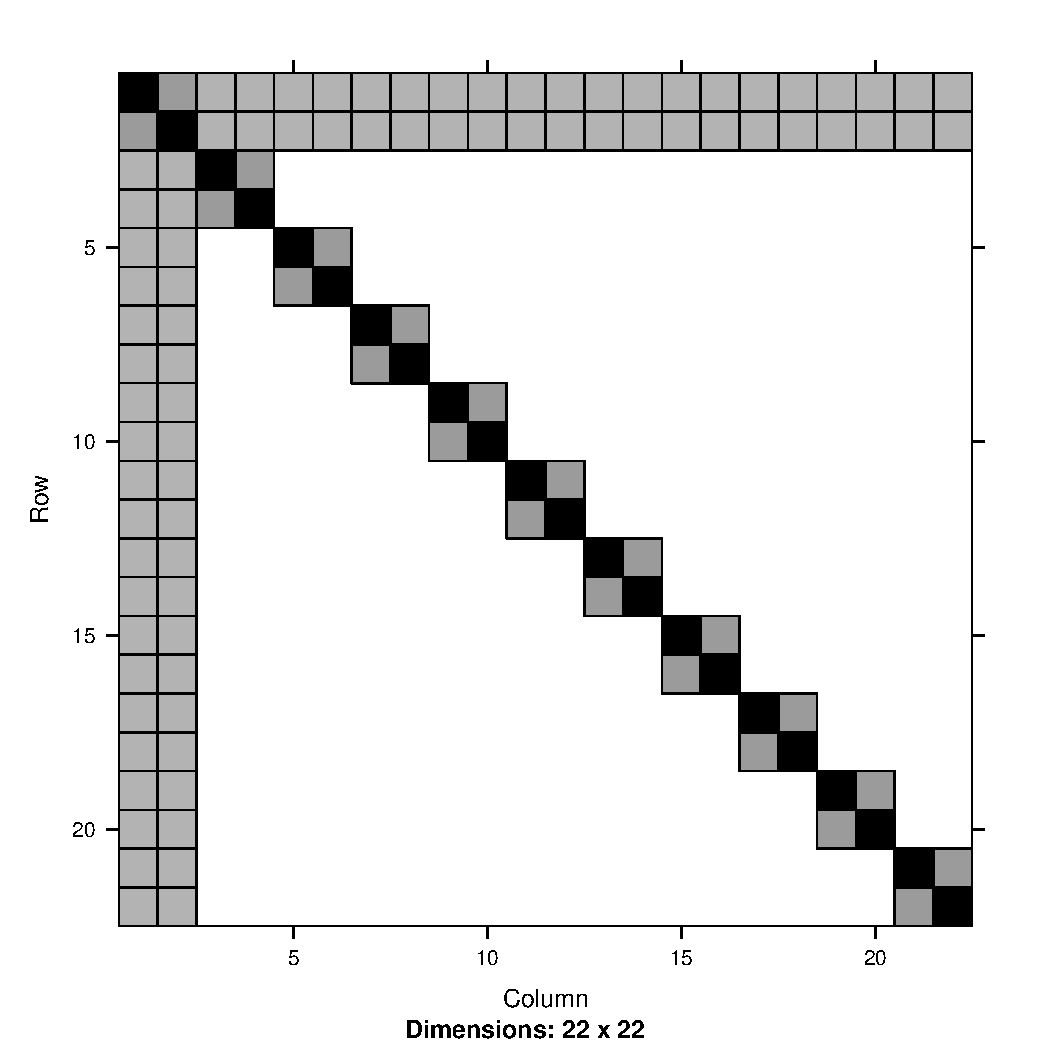
\includegraphics[scale=.25]{mX_mZ_mLambda.pdf}
	\end{figure}
		
	\begin{figure}[p]
		\caption{\tiny Covariance matrix -- Random effects before fixed effects}
		\label{fig:covrandomfixed}
		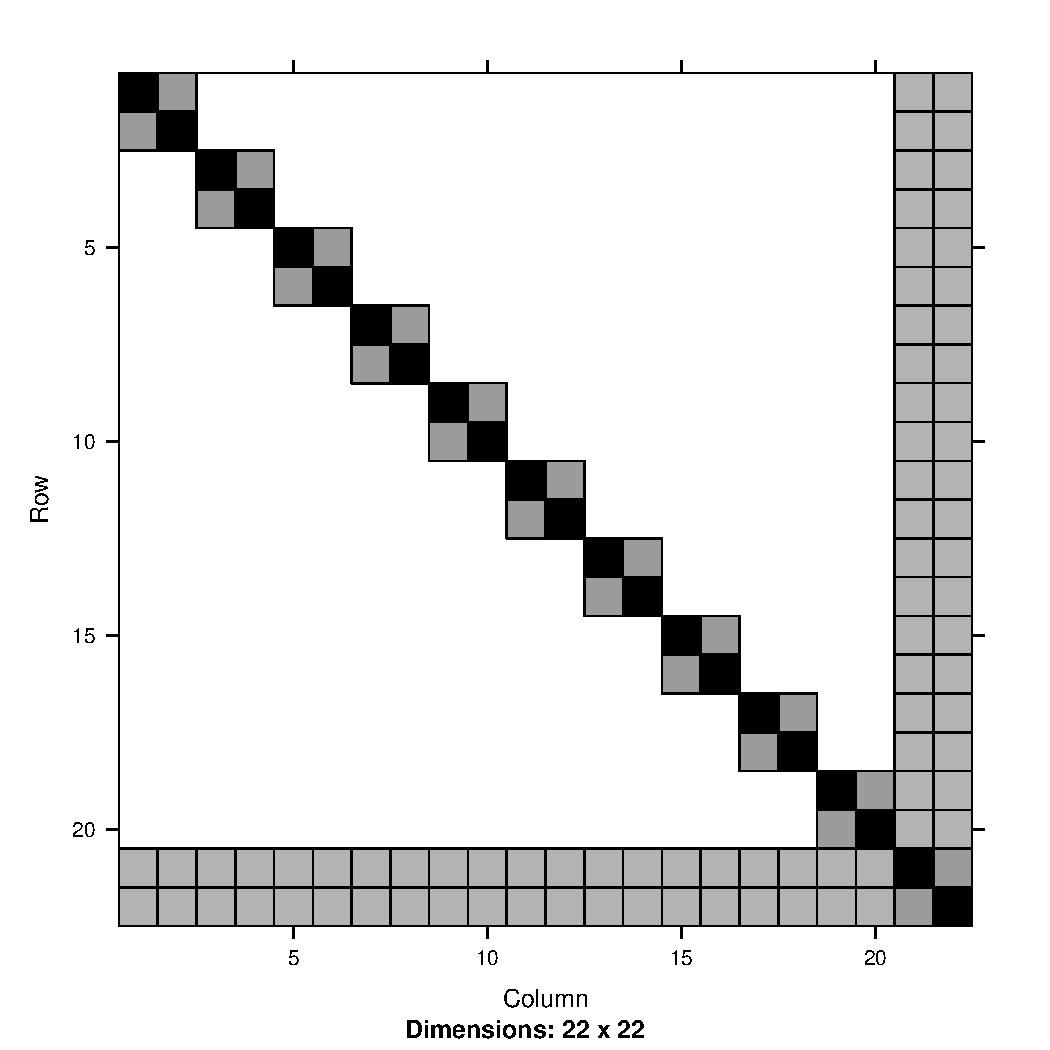
\includegraphics[scale=.25]{mZ_mX_mLambda.pdf}
	\end{figure}
							      				      			      			      			      	
	\begin{figure}[p]
		\caption{\tiny Cholesky factor -- Fixed effects before random effects}
		\label{fig:cholfixedrandom}
		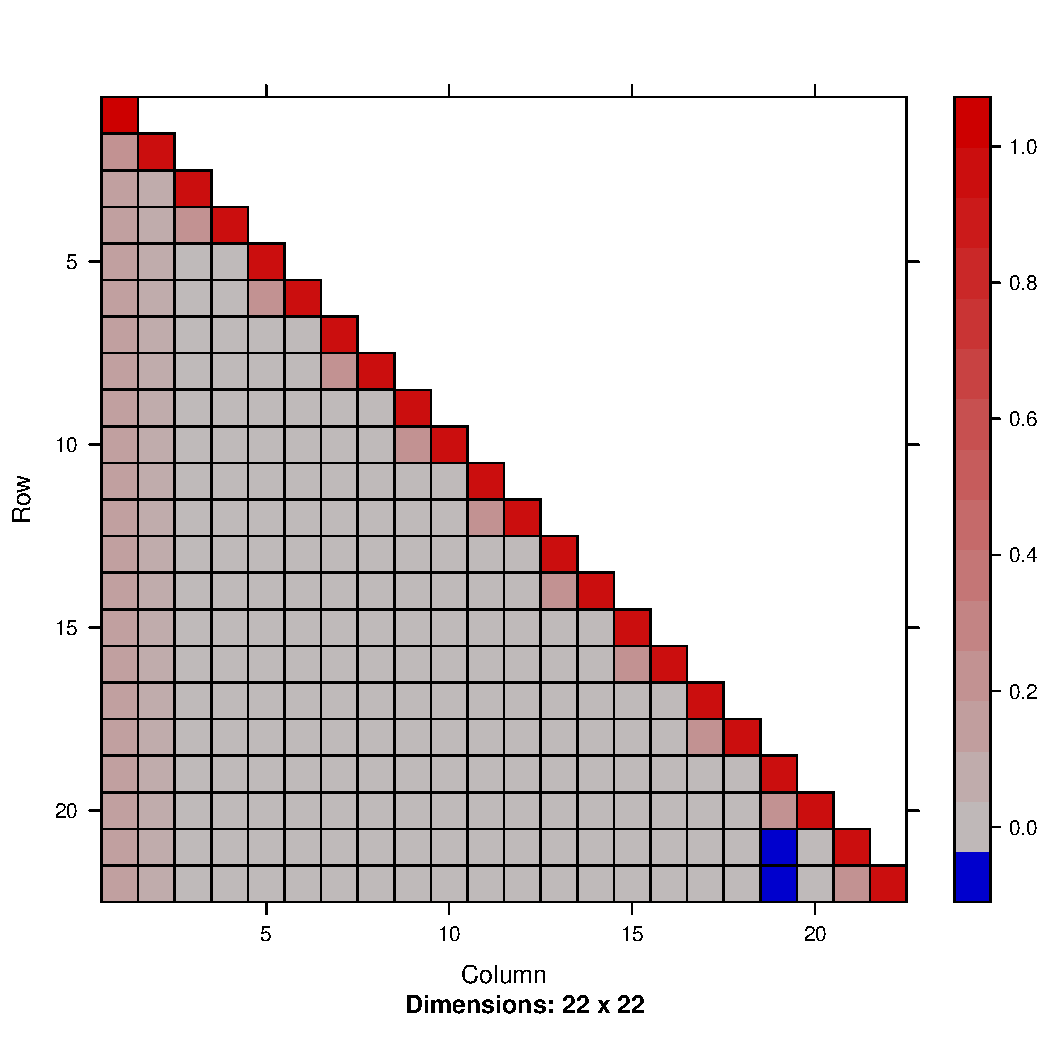
\includegraphics[scale=.25]{mX_mZ_cholesky.pdf}
	\end{figure}
		
	\begin{figure}[p]
		\caption{\tiny Cholesky factor -- Random effects before fixed effects}
		\label{fig:cholrandomfixed}
		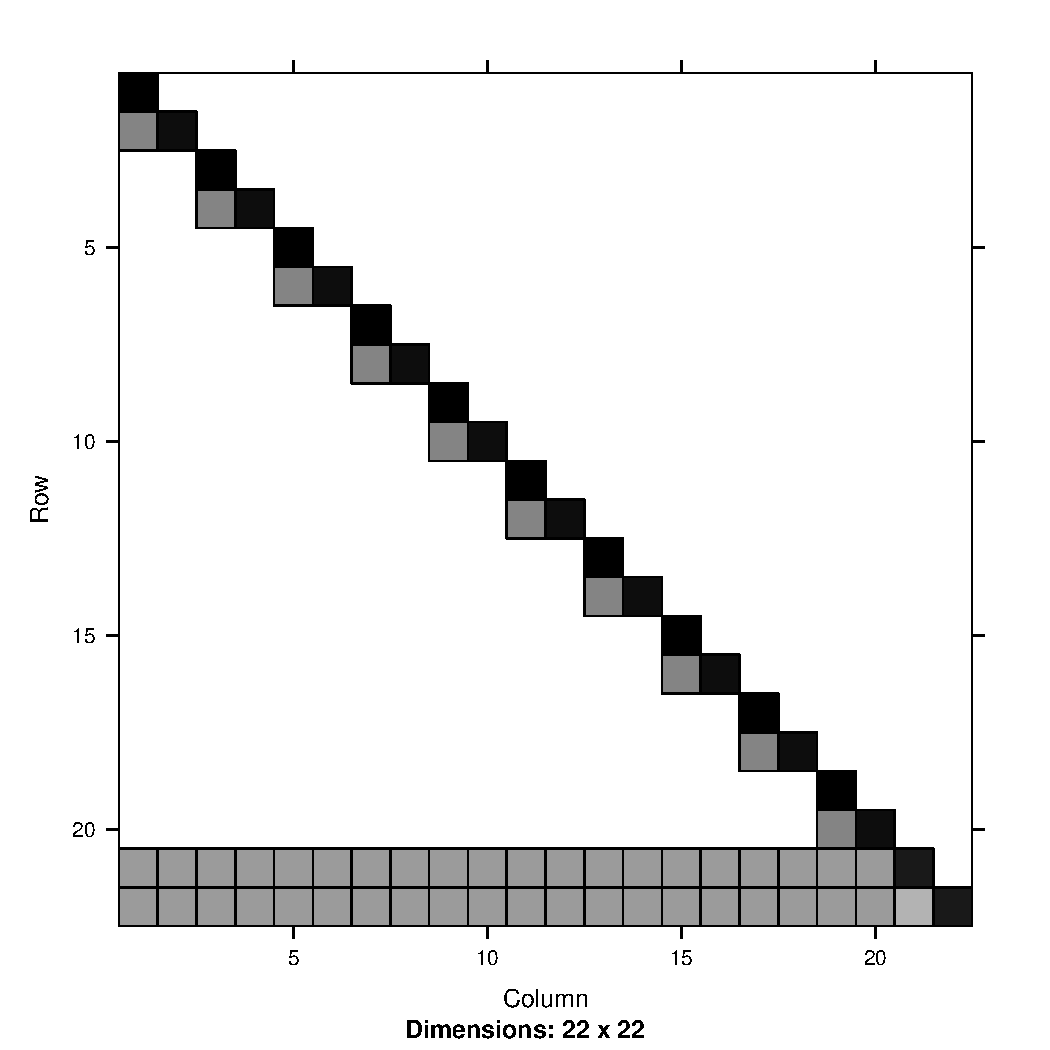
\includegraphics[scale=.25]{mZ_mX_cholesky.pdf}
	\end{figure}
		
	\subsubsection{Precision parameterisation $\mLambda = (\mR^\top \mR)^{-1}$}
			
	\noindent The second variant of the Gaussian Variational Approximation algorithm is similiar to the first, but
	instead of optimising the Gaussian variational lower bound with respect to $\vmu$ and the Cholesky factor
	$\mR$ of $\mLambda$, we instead optimise the Cholesky factor of the inverse of $\mLambda$ i.e. $\mLambda =
	(\mR \mR^\top)^{-1}$.
	
	The Gaussian variational lower bound in this parameterisation is
	\begin{align*}
		\log \underline{p}(\vmu, \mLambda; \vy) & = \quad \vy\mP\mC \vmu - \vp^\top \exp(\mC \vmu + \half \text{diag}(\mC \mLambda \mC^\top)) - \half \vmu^\top \mSigma^{-1} \vmu - \half \tr{(\mSigma^{-1} \mLambda)} \\
		                                        & \quad- \tfrac{p}{2} \log{(2 \pi)} + \half \log{|\mSigma^{-1}|} + \tfrac{p}{2} \log{(2 \pi)} + \tfrac{p}{2} - \log{|\mR|}                                             
	\end{align*}
			
	\noindent The derivative with respect to $\vmu$ is the same as that in the first variant of the algorithm, but 
	as the parameterisation of $\mLambda$ has changed, the  derivative with respect to $\mLambda$ becomes
	\begin{align*}
		\frac{\partial \log \underline{p}(\vmu, \mLambda; \vy)}{\partial \mLambda}
		  & = \hphantom{-}(\mLambda^{-1} + \mH)(-\mLambda \mR \mLambda) \\
		  & = -(\mI + \mH\mLambda)\mR\mLambda                           \\
		  & = - (\mR\mLambda + \mH\mLambda\mR\mLambda)                  
	\end{align*} 
			
	\noindent where $\mH = (\mP \mC)^\top \text{diag}(\exp(\mC \vmu + \half \mC \mLambda \mC^\top)) \mP \mC - \mSigma^{-1}$.
			
	\subsubsection{GVA fixed point}
			
	% Fixed point update of \mLambda
			
	This variant of the algorithm uses Newton-Raphson-like fixed point updates on the Gaussian variational lower
	bound. We optimise the same variational lower bound as in the covariance parameterisation above, using the
	derivatives below. The steps are presented in Algorithm \ref{alg:algorithm_nr} where	
	\begin{align*}
		\frac{\partial \log \underline{p}(\vmu, \mLambda; \vy)}{\partial \vmu}     & = \quad \mC^\top\vp \left [\vy - \mC\exp(\mC \vmu + \half \text{diag}(\mC \mLambda \mC^\top)) \right ] - \mSigma^{-1} \vmu \text{ and} \\
		\frac{\partial \log \underline{p}(\vmu, \mLambda; \vy)}{\partial \mLambda} & = -\mC^\top \text{diag}(\vp^\top \exp(\mC \vmu +\half \text{diag}(\mC \mLambda \mC^\top))) - \mSigma^{-1}.                             
	\end{align*}
	As this algorithm involves a simple Newton-Raphson style update step, it is computationally simple to
	implement, but potentially unstable as there is no adaptation of step size, as in L-BFGS-B.

	For efficiency, the inversion of $\mLambda$ within the algorithm was implemented using the block inverse 
	formula, where	the matrix was partitioned
	\[
		\mLambda =
		\begin{pmatrix}
			\mLambda_{\vbeta \vbeta} & \mLambda_{\vbeta \vu} \\
			\mLambda_{\vbeta \vu}^\top & \mLambda_{\vu \vu}
		\end{pmatrix}
	\]
	where $\mLambda_{\vbeta \vbeta}$ is the $p \times p$ approximation of the fixed effects covariance, $\mLambda_{\vbeta \vu}$ is the $p \times mb$
	approximation of the covariances between the fixed and random effects and $\mLambda_{\vu \vu}$ is the $mb \times mb$
	approximation of the random effects covariance.

	Sometimes in the course of  executing the algorithm, we observed numerical issues which had to be dealt
	with in order for the algorithm to successfully complete. If the block $\mLambda_{\vu \vu}$ cannot be inverted on an
	iteration, we reverted to $\vmu$ and $\mLambda$ from the previous iteration. If after updating $\vmu$
	any element is NaN, we reverted to the $\vmu$ and $\mLambda$ from the previous iteration. This greatly
	improved the stability of the algorithm.
	
	\begin{algorithm}
		\caption[Algorithm GVA NR]{Iterative scheme for obtaining optimal $\vmu$ and $\mLambda$
			given $\vy$, $\mC$ and $\vp$}
		\label{alg:algorithm_nr}
		\begin{algorithmic}
			\REQUIRE $\frac{\partial \log \underline{p}(\vmu, \mLambda; \vy)}{\partial \vmu} = \mP \mC (\vy - \mC^\top \exp(\mC \vmu + \half \text{diag}{(\mC \mLambda \mC^\top)})) - \mSigma^{-1} \vmu$.
			% Fit \vmu, \mLambda using Laplace approximation
			\WHILE{the increase in $\log{\underline{p}}(\vmu, \mLambda; \vy)$ is significant}
			% \vmu, \mLambda
			\STATE $\mLambda^{-1} = \left [ \mP^\top \mC^\top \exp(\mC \vmu + \half \text{diag}(\mC \mLambda \mC^\top)) \mC \mP \right ]$ \\ [1ex]
			Calculate \STATE $\mLambda \leftarrow \left (\mLambda^{-1} \right )^{-1}$  using the block inverse formula \\ [1ex]
			If $\mLambda_{\vu \vu}$ cannot be inverted in the above calculation, revert to $\vmu$ and $\mLambda$ from the previous iteration \\ [1ex]
			\STATE $\frac{\partial \log \underline{p}(\vmu, \mLambda; \vy)}{\partial \vmu} = -\mC^\top \text{diag}(\vp^\top \exp(\mC \vmu +\half \text{diag}(\mC \mLambda \mC^\top))) - \mSigma^{-1}$ \\ [1ex]
			\STATE $\vmu \leftarrow \vmu + \mLambda \left [ \frac{\partial \log \underline{p}(\vmu, \mLambda; \vy)}{\partial \vmu} \right ]$ \\ [1ex]
			If any element of $\vmu$ is NaN, revert to $\vmu$ and $\mLambda$ from the previous iteration
			\ENDWHILE
		\end{algorithmic}
	\end{algorithm}
			
	% Splines
			
	\section{Parameterisations and computational cost of Gaussian Variational Approximation approaches}
	\label{sec:param}
	\subsection{Covariance parameterisation of $\mLambda$}
	
	To ensure symmetry of $\mLambda$, we parameterise the optimisation problem in terms of $\mLambda$'s
	Cholesky factor  $\mLambda = \mR^\top \mR$. We optimise over the space $(\vmu, \overline{\mR})$, where $\vmu
	\in \R^{p + m}b$ and $\overline{\mR}$ is a lower-triangular $(p + mb) \times (p + mb)$ matrix. Then
			
	\begin{equation*}
		\mR_{ij} =
		\begin{cases}
			\exp(\overline{\mR}_{ij}), & i = j             \\
			\overline{\mR}_{ij},       & i > j             \\
			0,                         & \text{otherwise}, 
		\end{cases}
	\end{equation*}
			
	\noindent exponentiating the diagonal to ensure positive-definiteness of $\mR$. We parameterise $\mLambda$
	as $\mLambda = \mR \mR^\top$ so that is is guaranteed to be symmetric, and we only have $p(p-1)/2$ 
	parameters to deal with instead of $p^2$ parameters, some of which are constrained. 
	
	This parameterisation can lead to numeric overflow when the diagonals of $\overline{\mR}$ become moderately
	large, which can lead to singular matrices when attempting to invert $\mLambda$. We dealt with this by
	defining a piecewise function which is exponential for arguments less than $t$, and quadratic for arguments
	greater than or equal to $t$
	$$
	f(r_{ij}) =
	\begin{cases}
		e^{r_{ij}}, r_{ij} < t                   \\
		a r_{ij}^2 + b r_{ij} + c, r_{ij} \geq t 
	\end{cases}
	$$
	and then choosing the co-efficients $a$, $b$ and $c$ such that the function, first and second derivatives would
	agree at $r_{ij} = t$.
	
	To find the co-efficients $a$, $b$ and $c$, we solved the system of equations formed by repeatedly 
	differentiating the quadratic at $r_{ij} =  t$ and equating it with $e^t$
	$$
	\begin{array}{lllll}
		e^t & = & a t^2 & + \quad b t & + \quad c \\
		e^t & = &       & \quad 2a t  & + \quad b \\
		e^t & = &       &             & \quad 2a  \\
	\end{array}
	$$
	to obtain $a = e^t / 2$, $b = (1 - t) e^t$ and $c = [1 - t^2/2 - (1 - t) t] e^t$.
	
	We also addressed the overflow problem by working with the Cholesky factorisation of $\mLambda^{-1}$
	rather than $\mLambda$, allowing us to solve a system of equations rather than invert and multiply by a
	matrix, which is also faster and more numerically stable. We use knowledge of the regression  model we are
	fitting to specify a sparse matrix structure, greatly reducing the dimension of   the problem and thus
	improving both computational speed and numeric accuracy.
	
	% \noindent By noticing that the lower rows of the product depend on the higher rows of the Cholesky factor, we
	% observe that by re-ordering the fixed and random effects in $\mLambda$ so that the , we arrive at a covariance structure which is sparse in the first diagonal block. Thus the Cholesky factor of $\mLambda$ that we optimise over is as sparse as possible. This reduces the dimension of the optimisation problem we have to solve from
	% $\BigO(np^2)$ to $\BigO(np)$.
		
	Any symmetric matrix $\mLambda$ can be written as a product of its' Cholesky factors, $\mLambda =
	\mR \mR^\top$ where $\mR$ is lower triangular. $\mR$ is unique if $\mR_{ii} \geq 0$.
		
	\begin{align*}
		&\begin{pmatrix}
		\mR_{11}          & 0                                    & 0                                     \\
		\mR_{21}          & \mR_{22}                             & 0                                     \\
		\mR_{31}          & \mR_{32}                             & \mR_{33}                              
		\end{pmatrix}
		\begin{pmatrix}
		\mR_{11}          & \mR_{21}                             & \mR_{31}                              \\
		0                 & \mR_{22}                             & \mR_{32}                              \\
		0                 & 0                                    & \mR_{33}                              
		\end{pmatrix}
		\\
		=& \begin{pmatrix}
		\mR_{11}^2        &                                      & \text{symmetric}                      \\
		\mR_{21}\mR_{11} & \mR_{21}^2 + \mR_{22}^2 \\
		\mR_{31} \mR_{11} & \mR_{31}\mR_{21} + \mR_{32} \mR_{22} & \mR_{31}^2 + \mR_{32} ^2 + \mR_{33}^2 
		\end{pmatrix}.
	\end{align*}
	
	\noindent We exploit this structure. By interchanging the fixed and random effects in the design matrix $\mC = [\mX \mZ]$ to $\mC = [\mZ \mX]$, and re-ordering the dimensions of $\vmu, \mLambda$ and $\mSigma$ in the same manner, the independence between the
	blocks relating to the random effects in $\mZ$ induce sparsity in the Cholesky factor $\mR$ of
	$\mLambda^{-1}$, as can be seen in Figures \ref{fig:covfixedrandom}, \ref{fig:covrandomfixed},
	\ref{fig:cholfixedrandom} and \ref{fig:cholrandomfixed}. Thus the Gaussian $q(\vnu) \sim \N(\vmu, \mLambda)$ can be optimised over a space of dimension $\half p (p + 1) + pq + \half q (q + 1)$ rather than dimension
	$\half (p + mq) (p + mq + 1)$ as in the dense parameterisation. This leads to subtantial performance gains
	when $m$ is large, as is typically the case in problems of practical importance such as longitudinal or 
	clinical trials with many subjects or the application presented in Section \ref{sec:application}.
			
	By re-ordering the fixed and random effects in $\mLambda$, we end up with a covariance structure which is 
	sparse in the first diagonal block.
	
	\subsection{Precision parameterisation}
	
	We optimise over the space $(\vmu, \overline{\mR})$ as before, but now 
			
	\begin{equation*}
		\mR_{ij} =
		\begin{cases}
			\exp(-\overline{\mR}_{ij}), & i = j             \\
			\overline{\mR}_{ij},        & i > j             \\
			0,                          & \text{otherwise}, 
		\end{cases}
	\end{equation*}
		
	\noindent This new choice of parameterisation allows us to calculate $\half \text{diag}(\mC \mLambda
	\mC^\top)$ by solving the linear systems $\mR \va = \mC_{i}, i=1, \ldots, n$ for   $\va$ and then calculating
	$\va^\top\va$ where $\mC_{i} = $ the $i$th row of $\mC$, rather than calculating $\text{diag}(\mC \mLambda
	\mC^\top)$ directly.
		
	% TODO: We fixed this using safe-exp
	The implementation of these algorithms was not without its' challenges, chiefly numerical issues encountered during testing and verification of the accuracy of the model fitting. Using the exponential function to parameterise the main diagonal coupled with L-BFGS-B's unconstrained line search and \texttt{optim()}'s lack of robustness to infinities lead to many overflow problems which may have been lessened or dealt with entirely by using a function with a less aggressive growth rate, such as an appropriate piecewise quadratic.
		
	The main computational cost is the evaluation of the variational lower bound and its' derivatives. By
	virtue of their dimension, the expressions involving $\mLambda$ dominate the computational cost. The key
	term is $\frac{1}{2} \diag(\mC \mLambda \mC^\top)$. This can be naively calculate by ignoring the
	symmetry in the expression and simply calculating the product $\mC \mLambda \mC^\top$, taking $2 n
	\times (p + m b)^2$ floating point operations, and retaining the diagonal entries of the result. This is
	obviously wasteful, as the off--diagonal entries of the resulting product that has just been computed
	are immediately discarded.
		
	By parameterising $\mLambda$ in terms of its' Cholesky factors and realising that
		
	\[
		\mC \mLambda \mC^\top = \mC \mR \mR^\top \mC^\top
	\]
		
	\noindent and that
		
	\[
		\diag(\mC \mLambda \mC^\top)_{ii} = \mC_{i .} \mR \mR^\top \mC_{i .}^\top, 1 \leq i \leq n
	\]
		
	\noindent we can calculate the products $\mC_{i .} \mR, 1 \leq i \leq n$, using $n \times \frac{1}{2}(p + m
	b)(p + m b   + 1)$ floating point operations, and storing the results of the $i$th product in the $i$th
	element of the   vector $\va$ and then calculate $\diag(\mC \mLambda \mC^\top) = \va^\top \va$.
		
	Moreover, mixed models typically have sparse design matrices, allowing us to encode $\mR$ as a sparse matrix, and	further reduce   this depending on the model. For example, in the random intercept case, only the diagonals of the random effects block need to be non-zero, and hence the above expression can be calculated in
	$\BigO(n)$ floating point operations.
		
	% $\log |\mR|$ can be calculated using only $p + m b$ floating point operations, as $\mR$ is lower triangular.
		
	For the precision parameterisation, we observe that in this parameterisation
	\[
		\diag(\mC \mLambda \mC^\top)_{ii} = \mC_{i .} \mR^{-\top} \mR^{-1} \mC_{i .}^\top, 1 \leq i \leq n,
	\]
		
	\noindent and so by solving $\mR \va = \mC_{i .}^\top$ for $\va$ for all $i$ at a cost of $n \times
	\frac{1}{2} (p + m b) (p + m b + 1)$ floating point operations, and then calculating
	\[
		\diag(\mC \mLambda \mC^\top)_{ii} = \va^\top \va, 1 \leq i \leq n,
	\]
		
	\noindent we can then calculate $\diag(\mC \mLambda \mC^\top)$.
		
	As above, by using our knowledge of the model being fit we can encode $\mR$ sparsely to decrease
	the required   computation still further. In the random intercept model case, the computational cost will drop
	to   $n \times [m + \half{1}{2} p (p + 1) + p \times m b]$.
				
			\section{Numerical results}
			\label{sec:results}
					
			The accuracy of each model fitting algorithms presented in Section \ref{sec:gaussian} was assessed by
			comparing the approximating distribution of each parameter with the posterior distribution of Monte Carlo
			Markov Chain samples of that parameter. 1 million Monte Carlo Markov Chain samples were generated using Stan.
			The accuracy of examples of random intercept, random slope and spline models were evaluated using this method.
					
			\subsection{Simulated data}
					
			For each of these simulations, the model is as presented in Section \ref{sec:model}.
					
			Several common application scenarios were simulated and their accuracy evaluated. A random intercept model was simulated with $\vbeta = (2, 1)^\top$, $\rho = 0.5$, $m = 20$, $n_i = 10$ and $b = 1$. The results are
			presented in Table \ref{tab:accuracy_int}. A random slope model was simulated with $\vbeta = (2, 1)^\top$,
			$\rho = 0.5$, $m = 20$, $n_i = 10$ and $b = 2$. The results are presented in Table \ref{tab:accuracy_slope}.
			Spline model was fit to a data set generated from the function $3 + 3 \sin{(\pi x)}$ on the interval $[-1,
			1]$. The resulting model fits are presented in Figure \ref{fig:spline}.
					
			To assess the speed of each approach, a test case was constructed of a random slope model with $m=50$ groups,	each containing $n_i = 100$ individuals. A model was then fit to this data set ten times using each algorithm, and the results averaged. They are presented in Table \ref{tab:application_slope_speed}.

			\begin{table}
				\caption{Table of results - Speed}
				\label{tab:application_slope_speed}
				\begin{tabular}{|l|rr|}
					\hline
					Algorithm                            & Mean (seconds) & Standard deviation (seconds) \\
					\hline
					Laplace's method                     & 0.37 s         & 0.07 s                       \\
					GVA covariance parameterisation        & 2.04 s         & 1.24 s                       \\
					% Why is this slower?
					GVA inverse parameterisation & 0.38 s         & 0.66 s                       \\
					GVA fixed point                            & 0.05 s         & 0.07 s                       \\
					\hline
				\end{tabular}
			\end{table}

			% The stability of the algorithms was confirmed by running them on 10,000 different data sets that were randomly
			% generated after having initialised the random number generator with different seeds.
					
			Median accuracy of the algorithms was assessed by running them on 100 randomly generated data sets. The	results are presented in Figure \ref{fig:median_accuracy_intercept} and Figure
			\ref{fig:median_accuracy_slope}.
					
			% Figure: Median accuracy graph intercept
			\begin{figure}
				\begin{center}
					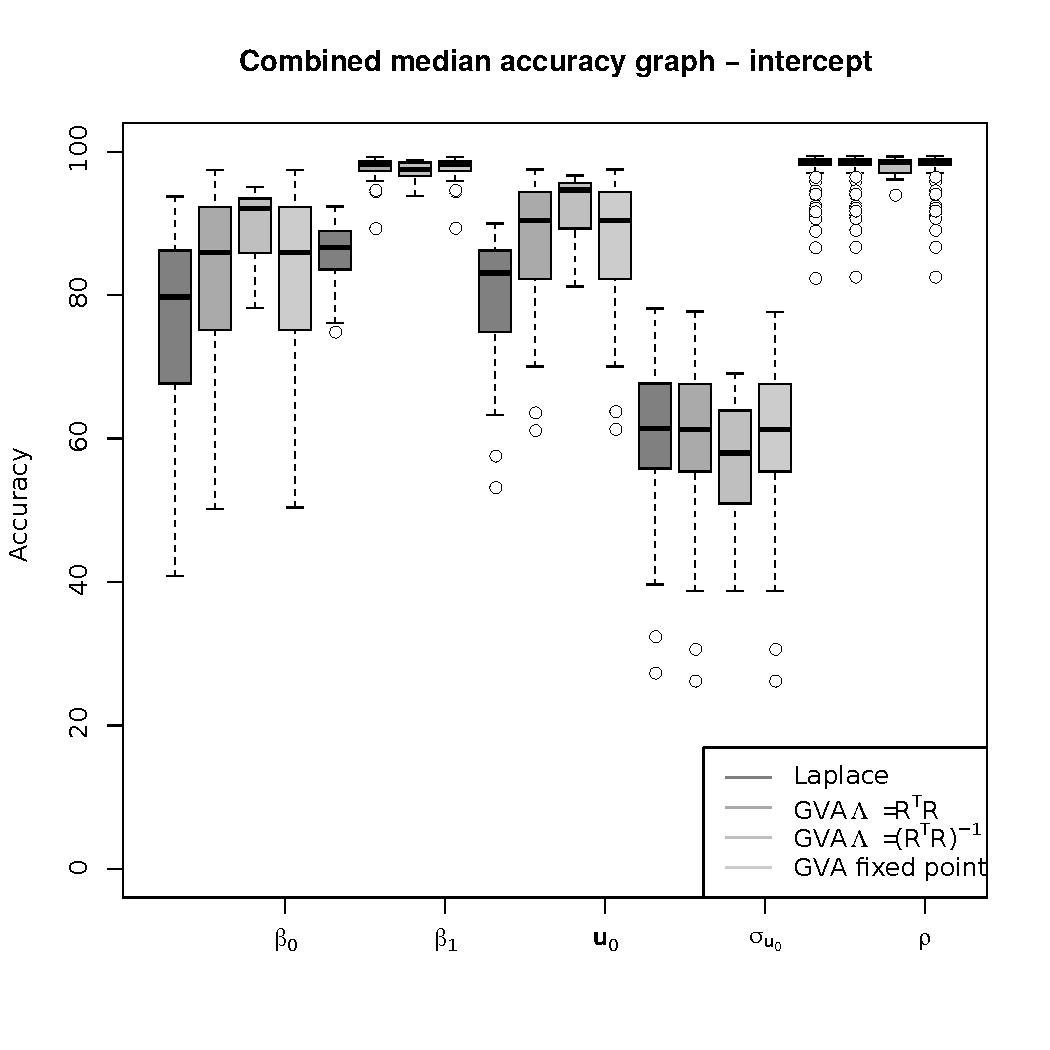
\includegraphics[width=0.7\textwidth, height=100mm]{code/results/median_accuracy_combined_intercept.pdf}
					\caption{Median accuracy of random intercept}
					\label{fig:median_accuracy_intercept}
				\end{center}
			\end{figure}
					
			% Figure: Median accuracy graph slope
			\begin{figure}
				\caption{Median accuracy of slope}
				\label{fig:median_accuracy_slope}
				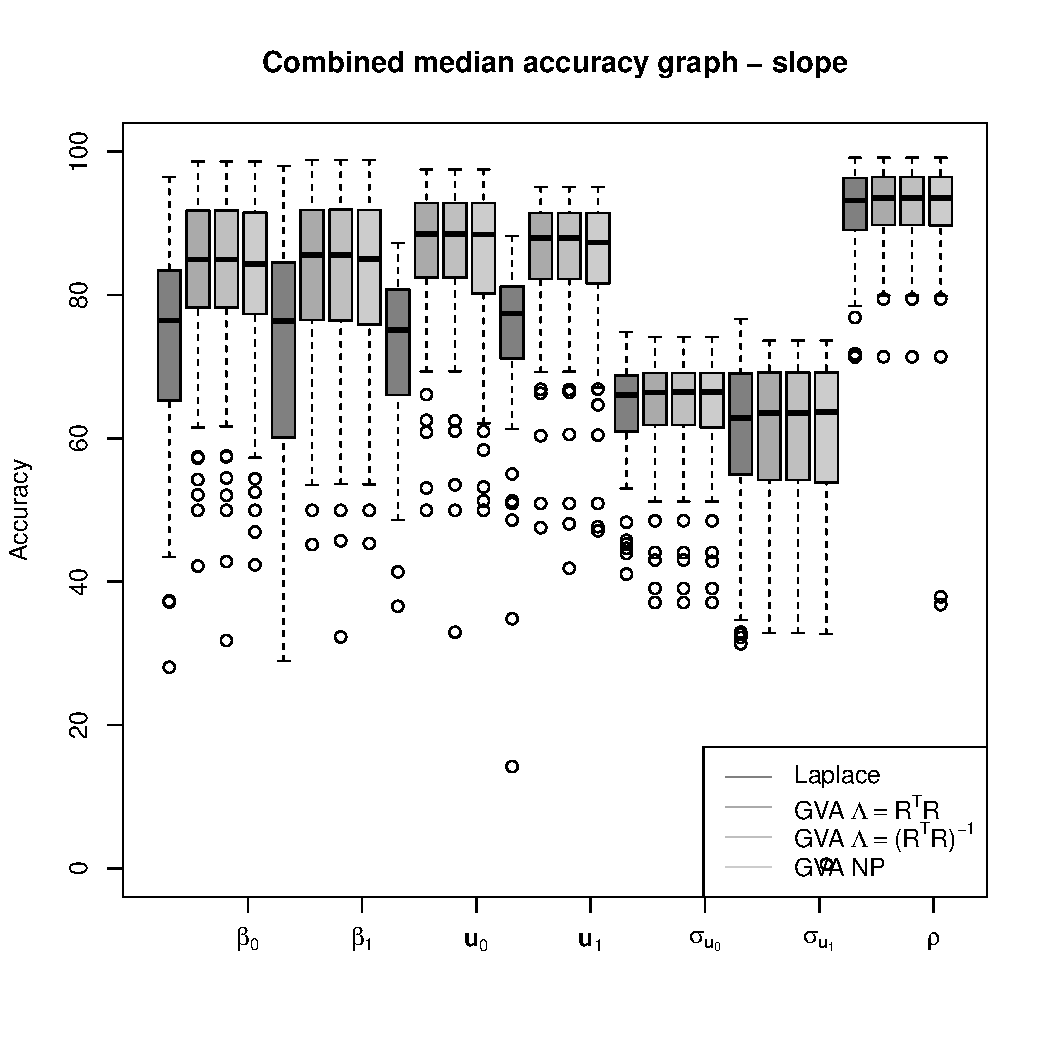
\includegraphics[width=120mm, height=120mm]{code/results/median_accuracy_combined_slope.pdf}
			\end{figure}
					
			% Table of accuracy results - intercept model
			\begin{table}
				\caption{Table of accuracy - Random intercept model}
				\label{tab:accuracy_int}
				\begin{tabular}{|l|rrrr|}
					\hline
					                   & Laplace's Method & GVA $(\mLambda = \mR \mR^\top)$ & GVA NP $(\mLambda = (\mR \mR^\top)^{-1})$ & GVA FP \\
					\hline
					$\vbeta_1$         & $85\%$           & $90\%$                          & $91\%$                                    & $90\%$ \\ 
					$\vbeta_2$         & $76\%$           & $98\%$                          & $99\%$                                    & $99\%$ \\ 
					Mean of $\vu$      & $81\%$           & $94\%$                          & $94\%$                                    & $94\%$ \\
					$\sigma^2_{\vu_1}$ & $66\%$           & $66\%$                          & $66\%$                                    & $66\%$ \\ 
					$\rho$             & $99\%$           & $99\%$                          & $99\%$                                    & $99\%$ \\ 
					\hline
				\end{tabular}
			\end{table}
					
			\begin{table}
				\caption{Table of accuracy - Random slope model}
				\label{tab:accuracy_slope}
				\begin{tabular}{|l|rrrr|}
					\hline
					                   & Laplace's Method & GVA $(\mLambda = \mR \mR^\top)$ & GVA $(\mLambda = (\mR \mR^\top)^{-1})$ & GVA FP \\
					\hline
					$\vbeta_1$         & 67\%             & 88\%                            & 88\%                                   & 88\%   \\
					$\vbeta_2$         & 70\%             & 89\%                            & 88\%                                   & 89\%   \\
					Mean of $\vu$      & 70\%             & 91\%                            & 91\%                                   & 91\%   \\
					$\sigma^2_{\vu_1}$ & 71\%             & 73\%                            & 73\%                                   & 73\%   \\
					$\sigma^2_{\vu_2}$ & 68\%             & 69\%                            & 69\%                                   & 69\%   \\
					$\rho$             & 91\%             & 90\%                            & 90\%                                   & 90\%   \\
					\hline
				\end{tabular}
			\end{table}
					
			% \begin{table}
			% \caption{Table of accuracy - Splines}
			% \label{tab:accuracy_spline}
			% \begin{tabular}{|l|l|}
			% \hline
			% Approximation & Accuracy \\
			% \hline
			% Laplace's Method & 0.969 \\
			% GVA & 0.969 \\
			% GVA NP & 0.969 \\
			% GVA NR & 0.969 \\
			% \hline
			% \end{tabular}
			% \end{table}
					
			\begin{figure}
				\label{fig:spline}
				\caption{Comparison of VB and MCMC spline fits with the true function}
				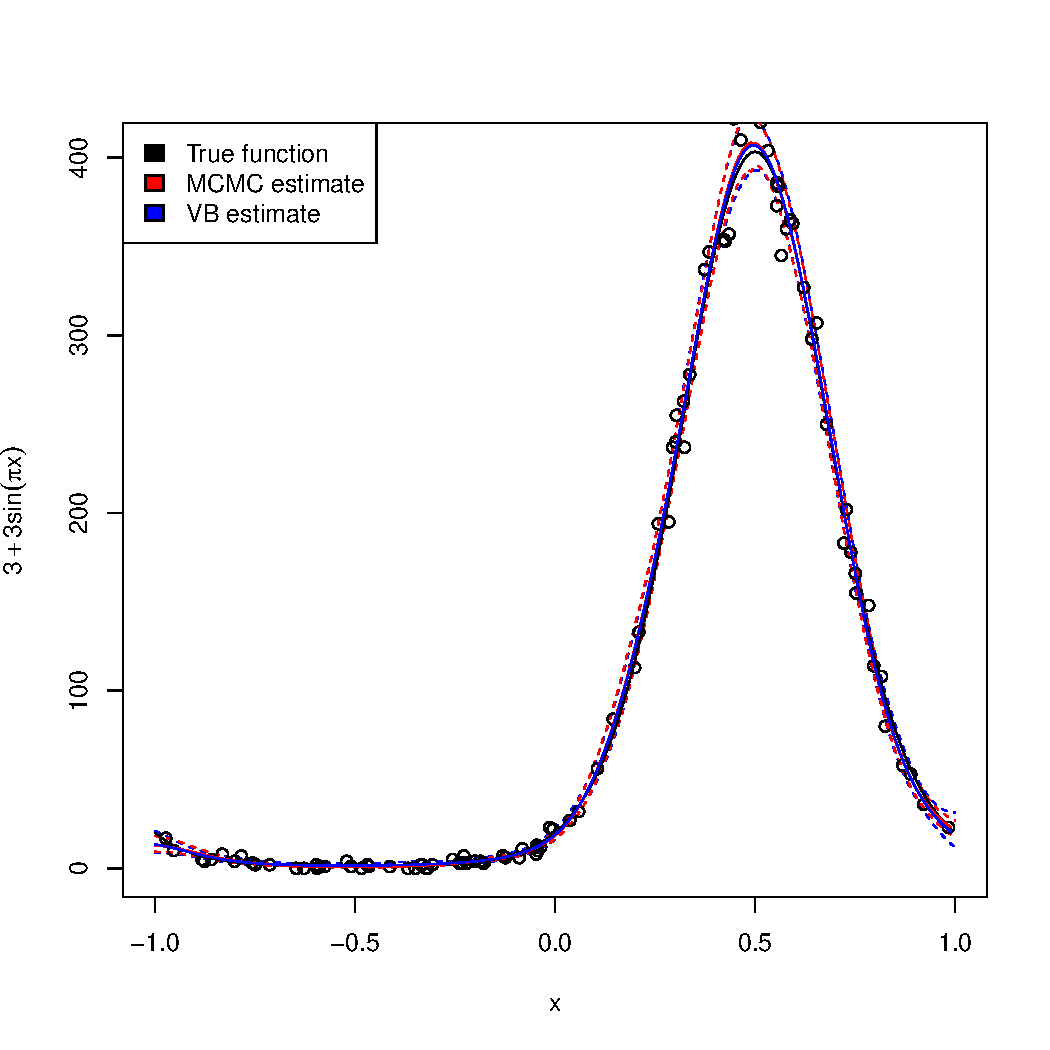
\includegraphics[width=100mm, height=100mm]{code/results/accuracy_plots_spline_gva2.pdf}
			\end{figure}
					
			% Graphs - exactly what sort of graphs do we need?
			% Median accuracy
			% Increase in lower bound
			% MCMC posterior, with approximating posterior for at least one or two of the
			% key parameters, such as, say, vbeta[2]
					
			\subsection{Numerical stability of the parameterisation}
			
			In the process of performing numerical experiments, we discovered that our model fitting software was 
			prone to numeric overflow due to the log link in our model and the exponentiation of the diagonals of the
			Cholesky factors in the covariance parameterisation of the Gaussian Variational Approximation of $\vnu$.
			
			We dealt with this difficulty by developing a 'safe exponential' parameterisation for the diagonals of the
			Cholesky factors. The parameterisation is exponential up to a threshold $t$, and then quadratic beyond that
			threshold.
			
			The stability of this scheme was tested by calculating the accuracy of the approximations fit with a range
			of safe exponential thresholds, the results of which are presented in Figure \ref{fig:stability_accuracy}.
			The variational approximation was found to be stable, with the accuracy largely insensitive to the choice of
			threshold.
			
			\begin{figure}
				\label{fig:stability_accuracy}
				\caption{Accuracy of approximation of parameters versus the safe exponential threshold}
				\includegraphics{code/stability_intercept.pdf}
			\end{figure}
			
			We repeated our numerical experiments with the new parameterisation, varying the threshold within reasonable
			bounds and found that the numerical experiments no longer resulted in overflow, and that the numerical accuracy
			of the approximation was still very good.
			
			The stability of the GVA algorithm with the parameterisation $\mLambda = (\mR^\top \mR)^{-1}$ depends on the
			threshold chosen for the safe exponential function. When the threshold is set to $2$, the algorithm is stable
			for all starting points within the grid except $6$. When the threshold is set to $\infty$, equivalent to using
			the naive $\exp$ parameterisation, the algorithm encounters numerical errors for every starting point on the 
			grid.
				
			\subsection{Stability of the GVA precision parameterisation algorithm for different starting points}
					
			The numerical stability of each fitting algorithm in Section \ref{sec:gaussian} was assessed by initialising
			each algorithm from a range of different starting points. Errors due to numerical instability and the fitted
			$\vmu$ were recorded for each starting point.
					
			A data set of 100 individuals in ten groups ($m=10$) was generated from a model with a fixed intercept and
			slope, and a random intercept. $\vmu$ was initialised from a grid of points on the interval $[-4.5, 5]$ for
			intercept and slope, spaced $0.1$ apart. The error counts are presented in Table
			\ref{tab:stability_results}. Plots of the starting locations which resulted in numerical errors when the
			fitting algorithm was run are presented in \ref{fig:stability_locations_gva}.
					
			\begin{table}
				\caption{Count of numerical errors for each algorithm during stability tests}
				\label{tab:stability_results}
				\begin{tabular}{|l|r|}
					\hline
					Algorithm                            & Error count \\
					\hline
					Laplace's algorithm                  & 12          \\
					GVA $\mLambda = \mR^\top \mR$        & 1,306       \\
					GVA $\mLambda = (\mR^\top \mR)^{-1}$ & 6           \\
					GVA NR fixed point                   & 992         \\
					\hline
				\end{tabular}
			\end{table}

			The GVA algorithm with the $\mLambda = (\mR \mR^\top)^{-1}$ parameterisation was less prone to
			instability due to starting point when the safe exponential parameterisation was used then when it was
			not used, as can be seen from Figure \ref{fig:stability_locations_gva}. % FIXME: Add error counts
					
			\begin{figure}
				\label{fig:stability_locations_gva}
				\caption{Starting locations which caused the GVA fitting algorithm to fail with numeric errors. The true model had fixed parameters $\vbeta = (2, 1)^\top$ and random intercepts. There were ten groups in the
					hierarchical model each	with ten individuals $(m=10, n_i=10)$}
				\includegraphics[scale=0.4]{code/safe_exp_stability.pdf}
				\includegraphics[scale=0.4]{code/no_safe_exp_stability.pdf}
			\end{figure}

			\subsection{Stability of the GVA fixed point algorithm for different starting points}

			The naive fixed point algorithm was extremely unstable for many starting points, as can be seen from
			Figure \ref{fig:stability_locations_nr}. The variant of the algorithm which checked whether the
			inversion of the $\mLambda_{\vu \vu}$ block of $\mLambda$ was performed successfully was much more
			stable, and did not suffer from any numeric errors at all over the range of starting points we tested.
			The algorithm is able to abort safely, and allow the Variational Bayes algorithm to update the other
			parameters before trying to fit the Gaussian component of the model again until the correct parameters
			are accurately estimated.

			\begin{figure}
				\label{fig:stability_locations_nr}
				\caption{Starting locations which caused the NR fitting algorithm to fail with numeric errors. The true model 						had fixed parameters $\vbeta = (2, 1)^\top$ and random intercepts. There were ten groups in the
					hierarchical model each	with ten individuals $(m=10, n_i=10)$}
				\includegraphics[scale=0.4]{code/local_solutions_gva_nr_error_locations_no_protections.pdf}
			\end{figure}
			
			\section{Application}
			\label{sec:application}
			
			\subsection{Poisson example without zero-inflated component -- Police stops}
			The data set used for this example was the police stop example from Chapter 15 of \citep{Gelman2007}.
			The model fit was
			\begin{align*}
				\vy_{ep}        & \sim \text{Poisson}(n_{ep} e^{\beta_0 + \beta_e \text{ethnicity}_e + \alpha_{c} \text{crime} + \vu_p}), \\
				\valpha				& \sim \N(0, \sigma_\valpha^2),	\\
				\vbeta        & \sim \N(0, \sigma_\vbeta^2), \text{ and }\\
				\vu_p         & \sim \N(0, \sigma_\vu^2)
			\end{align*}
			where $p$ is the $p$-th precinct, and $e$ is the $e$-th ethnicity (blacks, hispanics or whites), and $c$ is
			the $c$-th category of crime (violent crimes, weapons crimes, propery crimes, drug crimes). The random 
			intercepts $u_p$ allow for variation in the base rates of stops across precincts,
			the co-efficients $\beta_j$ measure the effect of ethnicity on the rate of police stops and
			the co-efficients $\alpha_k$ measure the effect of each type of crime on the rate.
			The model finds the relationship between the number of police stops in each precinct and 
			ethnicity	for each type of crime.
			
			The model was fit using the GVA algorithm with the $\mLambda = (\mR^\top \mR)^{-1}$ parameterisation, using
			the prior $a_\rho = 3$, $b_\rho = 1$ on $\rho$. Accuracy of the approximation was assessed by comparing the
			fitted distribution for each parameter to a kernel density estimate of the parameter's distribution from
			1 million samples from the equivalent model fitted using Stan. The results are presented in Table
			\ref{tab:application_police_stops}. Figure \ref{fig:police_stops}
			
			\begin{figure}\label{fig:police_stops}
			\caption{Accuracy of parameter estimates for police stops}
			\includegraphics[scale=0.3]{code/results/accuracy_plots_application2_GVA_inv_par-highlights-nup.pdf}
			\end{figure}

			% Table of results
			\begin{table}
				\caption{Table of results - Police stops}
				\label{tab:application_police_stops}
				\begin{tabular}{|l|rrrr|}
					\hline
					Covariate                     & Posterior Mean & Lower 95\% CI & Upper 95\% CI & Accuracy \\
					\hline
					Intercept [African-Americans] & 4.04          & 3.98           & 4.07          & 82.4\%   \\
					$\beta_2$ [hispanics]         & -0.45         & -0.46          & -0.43         & 98.1\%   \\
					$\beta_3$ [whites]            & -1.38         & -1.40          & -1.37         & 98.5\%   \\
					$\alpha_1$ [weapons crimes]   & 0.58          & 0.57           & 0.59          & 89.2\%   \\
					$\alpha_2$ [property crimes]  & -0.19         & -0.21          & -0.17         & 92.2\%   \\
					$\alpha_3$ [drug crimes]      & -0.750        & -0.77          & -0.73         & 94.9\%   \\
					Random intercept              & 1.321         & -0.190         & 2.202         & 86.7\%   \\
					$\sigma^2_{\vu}$              & 8.57          & 1.02           & 24.35         & 49\%     \\
					\hline
				\end{tabular}
			\end{table}
			
			% Table of speeds
			\begin{table}
				\caption{Table of speeds - Police stops}
				\label{tab:police_stop_speeds}
				\begin{tabular}{|ll|}
					\hline
					Algorithm & Time  in seconds \\
					\hline
					Laplace & 0.24 \\
					GVA covariance parameterisation & 6.02 \\
					GVA inverse paramaterisation & 3.92 \\
					GVA fixed point & 0.18 \\
					\hline
				\end{tabular}
			\end{table}
			
			% TODO: You need to describe the data set and the model.
			\subsection{Zero--inflated example -- Cockroaches in Apartments data set from Gelman}
			The model described in this section was fit
			 to the cockroach data set from \S 6.7 of \citep{Gelman2007}, taken from a study
			on the effect of integrated pest management in controlling cockroach levels in urban apartments. The data
			set contains data on 160 treatment and 104 control apartments, along with the response $y_i$ in each
			apartment of the number of cockroaches caught in a set of traps. The apartments had the traps deployed for
			different numbers of days, referred to as trap days, which was handled by using a log offset
			\citep{Agresti2002}. The predictors in the data set included the pre-treatment roach level, a treatment
			indicator, the time of the observation and an indicator for whether the apartment is in a senior building
			restricted to the elderly.
					
			In the example application presented in this paper, the zero component represents an apartment completely free of roaches, while the non-zero component represents an apartment where roaches have been able to live and reproduce, possibly in spite of pest control treatment aimed at preventing them from doing so.

			The model fit was
			\begin{align*}
				y_i &= \begin{cases}
				0 \phantom{-} \text{if} \phantom{-} R_i = 0 \\
				\Poisson(e^{\mX_i \vbeta + \mZ_i \vu}) \phantom{-} \text{if} \phantom{-} R_i = 1,
				\end{cases} \\
				R_i &\sim \Bernoulli(\rho), \\
				\rho &\sim \Beta(a, b), \\
				\vbeta &\sim \N(\vzero, \sigma^2_\vbeta \mI), \\
				\vu &\sim \N(\vzero, \mSigma), \text{and} \\
				\mSigma &\sim \text{Inverse-Wishart}(\mPsi, v)
			\end{align*}
			with prior parameters $a = 1$, $b = 1$, $\sigma^2_\vbeta = 10^5$, $\mPsi = 10^{-5} \mI$ and $v = 2$.
			These priors were chosen to be vaguely informative for the variance components and a uniform prior for
			the zero-inflation proportion latent variable $\rho$. The fixed effects covariates included in the
			model were time in days and time in days $\times$ pest control treatment. A random intercept to account
			for variation between the apartment buildings was included.
					
			The GVA algorithm with the $\mLambda = (\mR^\top \mR)^{-1}$ parameterisation was used to fit a random
			intercept model to the Roaches data set provided by Andrew Gelman. The fitted co-efficients and accuracy
			results are presented in Table \ref{tab:application_roaches}.
					
			%       lci  uci
			% 1  3.179 3.157 3.201
			% 2 -0.046 -0.053 -0.039
			% 3 -0.420 -0.434 -0.406
			% 1 -0.976 -1.015 -0.936
			% 2 -0.309 -0.323 -0.295
			% 3 -0.947 -0.963 -0.930
			% 4 -2.129 -2.384 -1.874
			% 5 -3.230 -3.490 -2.970
			% 6 -3.099 -3.404 -2.794
			% 7 -1.290 -1.326 -1.255
			% 8 -0.956 -0.991 -0.921
			% 9 -2.404 -2.600 -2.209
			% 10 -1.076 -1.123 -1.029
			% 11 -1.079 -1.107 -1.052
			% 12 -1.681 -1.737 -1.624
					
			%> round(cbind(fit1$vmu, lci, uci), 3)
			% fit1$a_rho
			% [1] 377.2375
			% > fit1$b_rho
			% [1] 152.7625
					
			\begin{table}
				\caption{Table of results - Roaches}
				\label{tab:application_roaches}
				\begin{tabular}{|l|rrrr|}
					\hline
					Covariate          & Posterior Mean & Lower 95\% CI & Upper 95\% CI & Accuracy \\
					\hline
					Intercept          & 3.42						& 3.2 					& 3.65          & 95\%     \\
					Time               & $-$0.14        & $-$0.05       & $-$0.02       & 96\%     \\
					Time:Treatment     & $-$0.31        & $-$0.43       & $-$0.14       & 96\%     \\
					Random intercept   & $-$1.60        & $-$1.71       & $-$1.49       & 90\%     \\
					$\sigma^2_{\vu_1}$ & 3.29           & 2.02          & 8.48          & 63\%     \\
					$\rho$             & 0.51           & 0.50          & 0.55          & 62\%     \\
					\hline
				\end{tabular}
			\end{table}
					
			\begin{figure}
				\caption{Accuracy graphs for roach model}
				\label{fig:accuracy_roach}
				\centering
				% \includepdf[width=75mm,height=75mm,pages={1,2,3,16},nup=2x2]{code/results/accuracy_plots_application_GVA2.pdf}
				\begin{tabular}{@{}c@{\hspace{.5cm}}c@{}}
				\includegraphics[scale=0.3]{code/results/accuracy_plots_application_GVA_inv_param-highlights-nup.pdf}
				\end{tabular}
			\end{figure}
					
			\subsection{Example - Biochemists}
			The model described in this section was fit to the biochemistry data set analysed by
			\cite{10.2307/2579146}. The sample was taken from 915 biochemistry graduate students. The outcome
			$\vy_i$ is the number of articles published in the last three years of the PhD. The covariates were the
			gender of the student, coded $1$ for female and $0$ for male, the marital status of the student ($1$ for
			married, $0$ for unmarried), the number of children under age six and the prestige of the PhD program.

			In this example application, the zero component represents the number of biochemists who did not publish
			any articles during the last three years of their PhD. Examination of the data reveals that this number
			is higher than would be expected if the data followed a purely Poisson distribution -- 30\% of
			biochemistry graduate students published no articles in their final years whereas a Poisson distribution
			would predict only 18\%. This justifies our choice of model.

			The model fit was
			\[
				y_i = \begin{cases}
				\begin{array}{ll}
				0 &\phantom{-} \text{if} \phantom{-} R_i = 0, \\
				\Poisson(e^{\vbeta_1 + \vbeta_2 \text{female} + \vbeta_3 \text{married} + \vbeta_4 \text{children under age 6} + \vbeta_5 \text{PhD}}) &\phantom{-} \text{if} \phantom{-} R_i = 1,
				\end{array}
				\end{cases}
			\]


			\noindent with priors
			\begin{align*}
			R_i &\sim \Bernoulli(\rho), \\
			\rho &\sim \Beta(A, B), \text { and } \\
			\vbeta &\sim \N(0, \sigma_\vbeta^2 \mI)
			\end{align*}

			\noindent with $A=1$, $B=1$ and $\sigma_\vbeta^2 = 10,000$. The model was fit using the GVA inverse parameterisation algorithm. The resulting model fit is presented in Table \ref{tab:biochemists_results}
			The accuracy of the parameter estimates is presented in Figure
			\ref{fig:biochemists}. As this is a fixed effects model with a large number of samples relative to the
			number of parameters being fit, we are able to estimate all of the parameters with great accuracy.

			\begin{figure}
			\label{fig:biochemists}
			\caption{Accuracy of the approximations of the parameters fit to the biochemists data}
			\includegraphics[scale=0.3]{code/results/accuracy_plots_application_biochemists_GVA_inv_param-nup.pdf}
			\end{figure}

			\begin{table}\label{tab:biochemists_results}
			\caption{}
			\begin{tabular}{|l|rrrr|}
				\hline
				Covariate          & Posterior Mean & Lower 95\% CI & Upper 95\% CI & Accuracy \\
				\hline
				Intercept & 0.86 & 0.65 & 1.06 & \\
				Female & -0.18 & -0.29 & -0.08 &  \\
				Married & 0.06 & -0.05 & 0.18 & \\
				Children under age 6 & -0.08 & -0.15 & -0.01 & \\
				PhD & 0.03 & -0.02 & -0.01 & \\
				\hline
			\end{tabular}			
			\end{table}
			
			\subsection{Example - Owls}
			The model described in this section was fit to the Owls data set from taken from \cite{zuur_mixed_2009}.
			The sample was 599 observations of owls grouped across 25 nests.The fixed covariates
			fit in the model were food treatment (Deprived or Satiated) and arrival time, a continuous covariate.
			The variation between the 25 different nests sampled from was modelled by a random intercept
			$\vu$.

			The model fit was
			\[
			y_i = R_i e^{\vbeta_1 + \vbeta_2 \text{Satiated} + \vbeta_3 \text{Arrival Time} + u_n}
			\]
			where $n$ is the $n$-th nest, with priors
			\begin{align*}
			R_i &\sim \Bernoulli(\rho), \\
			\rho &\sim \Beta(A, B), \\
			\vbeta &\sim \N(\vzero, \sigma_\vbeta^2 \mI), \\
			\vu &\sim \N(0, \sigma_\vu^2), \text { and } \\
			\sigma_\vu^2 &\sim \text{Inverse-Gamma}(s, t).
			\end{align*}
			where $\sigma_\vbeta^2=10,000$, $A=1$, $B=1$, $s=10^{-2}$ and $r=10^{-2}$.

			The model was fit using the GVA inverse parameterisation algorithm. The accuracy of the parameter
			estimates is shown in Figure \ref{fig:owls}. The variance component
			The runtime of the algorithms is shown in Table
			\ref{tab:owls_times}. We draw attention to the difference in run-times between the covariance and
			inverse parameterisations -- the inverse parameterisation is 

			\begin{figure}
			\caption{Accuracy of the approximations of the parameters fit to the Owls data}
			\label{fig:owls}
			\includegraphics[scale=0.3]{code/results/accuracy_plots_application_owls_GVA_inv_param-highlights-nup.pdf}
			\end{figure}

			\begin{table}\label{tab:owls_results}
			\begin{tabular}{|l|rrrr|}
				\hline
				Covariate          & Posterior Mean & Lower 95\% CI & Upper 95\% CI & Accuracy \\
				\hline
				Intercept & \\
				Female & \\
				Married & \\
				Children under age 6 & \\
				PhD & \\
				\hline
			\end{tabular}			
			\end{table}

			\begin{table}
			\caption{}
			\label{tab:owls_times}
			\begin{tabular}{|l|r|}
			\hline
			Algorithm & Time in seconds \\
			\hline
			Laplace & 0.988 \\
			GVA covariance parameterisation & 46.014 \\
			GVA inverse parameterisation & 2.056 \\
			GVA fixed point & 0.580 \\
			\hline
			\end{tabular}
			\end{table}

			\section{Discussion}
			\label{sec:discussion}
					
			We have described a Variational Bayes approximation to Zero-Inflated Poisson regression models which allows
			such models to be fit with considerable generality. We have also devised and extensively tested a number of
			alternative approaches for fitting such models, and extended one of these alternative approaches with a new
			parameterisation. Using MCMC methods as the gold standard to test against, we have assessed the accuracy and
			computational speed of these algoritms.
					
			The use of Mean Field Variational Bayes allows estimation of Bayesian ZIP models in a fraction of the time taken to fit the same model using even the best MCMC methods available, with only a small loss of accuracy.
			This is of great utility in applications where speed matters, such as model selection or when applied
			statisticians are choosing amongst many candidate models, as is typical in practice.
					
			The new parameterisation of Gaussian Variational Approximation using the Cholesky factorisation of the inverse of $\mLambda$ presented in Section \ref{sec:param} provides significant advantages.  It is well known that the inverse of a sparse matrix need not be sparse. 

			Mixed models have covariance matrices with a block structure, due to the dependence structure of the
			random effects. The precision parameterisation presented in this chapter is able to preserve this
			sparsity within the structure of the Cholesky factors of the inverses of the covariance matrices use in
			the variational lower bound by re-ordering the rows and columns of the matrices so that the random
			effects blocks appear first. The Owls example presented in this chapter shows the computational
			advantages of this approach when the number of groups $m$ in the model is large (m=27 in this case) --
			as the covariance parameterisation takes 46 seconds to fit whereas the inverse parameterisation only
			takes 3 seconds. This clearly demonstrates advantage of using sparsity to reduce the dimension of the
			optimisation problem to be solved when models are being fit -- as only the non-zero values in the
			covariance matrices need to be optimised over. This allows models to be fit more quickly, and with
			greatly improved numerical stability and without loss of accuracy.

			While all of the fitting algorithms presented in this chapter except the Laplace's approximation
			algorithm were able to fit ZIP random and fixed effects models with high accuracy, and the 
			Gaussian inverse parameterisation and fixed point algorithms were able to do so at high speed, they 
			could be numerically unstable depending on the data the model was being fit to and their starting points.
			In the case of the Gaussian inverse parameterisation algorithm, the source of the problem was tracked down
			to the exponential used in the parameterisation of the diagonal of the Cholesky factor of the precision
			matrix combined with the exponential that arises in the derivation of the Gaussian variational lower
			bound for Poisson mixed models -- leading to frequent numeric overflows during the fitting process. This
			problem, once discovered, was mitigated by replacing the exponential parameterisation of the diagonal
			of the Cholesky factor with a piecewise function which is exponential beneath a threshold and quadratic
			above that threshold. This was shown to greatly increase the numeric stability of the GVA inverse
			parameterisation for a range of starting points.

			Stability fixes.

			Cockroaches - few fixed covariates, random intercept for apartment buildings, zero-inflation
			Police stops - Pure Poisson model, no zero-inflation, random intercept for precincts/locality
			Biochemists - Zero-inflated, fixed effects
			Owls - Zero-inflated, random intercepts for nests, large number of nests, able to estimate variance 
			component very accurately
				
			Some of the algorithms which we experimented with were found to be very sensitive to their starting points.
			While these algorithms are typically initialised with a starting point as close as possible to the final
			solution, this gives some sense of the stability of each algorithm.
					
			This article presents the essential ideas necessary for a performant implementation implementing model fitting
			for ZIP regression models.%, but the performance would be even better if our algorithm was re-implemented in a
			%compiled language with good numeric libraries such as C++ with Eigen.
			The majority of the performance
			improvements over existing approaches come from avoiding unneccessary matrix inversion, which is a
			computationally expensive and numerically unstable process taking $\BigO(p^3)$ flops, and from constructing and 
			calculating	with sparse matrices. The gains of these approaches, particularly from sparse matrix techniques, 
			can be difficult to fully realise in R without expert knowledge of the underlying implementation and libraries.
					
			Our application of these ideas to Andrew Gelman's data showed that the new parameterisation very effectively
			speeds up fitting zero-inflated mixed models to real world data with a large number of groups, while still
			maintaining excellent accuracy versus an MCMC approach. This demonstrates the applicability of the ideas
			presented within this paper to real world data sets.
					
			\newpage
			\section{Appendix} 
			% TODO: Mean field updates?
			\subsection{Calculation of the Variational Lower bound}
			% Where are the priors for \vbeta and \vu
					
			The variational lower bound is equal to $\bE_q[\log{p(\vy, \vtheta)} - \log{q(\vtheta)}] = T_1 + T_2 + T_3$,
			where
			% This is the new T_1
			$$
			\begin{array}{rl}
				T_1 & = \quad \bE_q[\log{p(\vy, \vnu)} - \log{q(\vnu)}]                                                                                                                                                  \\
				    & = \quad \vy \mP \mC \vmu - \vp^\top \exp{\left[ \mC \vmu + \half \text{diag} (\mC \mLambda \mC^\top) \right]} - \vone^\top\log \Gamma{(\vy + \vone)}                                               \\
				    & \quad + \frac{p + m}{2} (1 + \log{2 \pi}) + \half \log{|\mLambda|},                                                                                                                                \\
				T_2 & = \quad \bE_q \left[ \log p(\mSigma_{\vu \vu}) - \log q(\mSigma_{\vu \vu}) \right]                                                                                                                 \\
				    & = \quad \bE_q \big[ v/2(\log |\Psi| - \log |\Psi + \vmu_\vu \vmu_\vu^\top + \mLambda_{\vu \vu}|) + \half \log 2 + \half \log|\mSigma_{\vu \vu}| + \log \Gamma_{p+1}(v/2) - \log \Gamma_{p}(v/2)    \\
				    & \quad + \half \tr((\vmu_{\vu} \vmu_{\vu}^\top + \mLambda_{\vu \vu}) \mSigma_{\vu \vu}^{-1}) \big]                                                                                                  \\
				    & = \quad v/2\big(\log |\Psi| - \log |\Psi + \vmu_\vu \vmu_\vu^\top + \mLambda_{\vu \vu}|\big) + \half \log 2 + \half \bE_q \log |\mSigma_{\vu \vu}| + \log \Gamma_{p+1}(v/2) - \log \Gamma_{p}(v/2) \\
				    & \quad + \half \tr\big(\mI_m + \Psi(\Psi+ \vmu_\vu \vmu_\vu^\top + \mLambda_{\vu \vu})^{-1}/(v + p + 2)\big)                                                                                        \\
				T_3 & = - \vp^\top \log \vp - (\vone - \vp)^\top \log (\vone - \vp) - \log \Beta (\alpha_\rho, \beta_\rho) + \log \Beta (\alpha_q, \beta_q)                                                              
			\end{array}
			$$
					
			\noindent with $\bE_q \log |\mSigma_{\vu \vu}| = m \log 2 + \log \left | \Psi + \vmu_\vu \vmu_\vu^\top + \mLambda_{\vu \vu} \right | + \sum_{i=1}^m \Psi \left ( \frac{v - i + 1}{2} \right )$

			\section{Appendix}
			\subsection{Derivatives for Laplace-Gaussian Variational Approximation}
			\label{sec:appendix_derivatives_laplace}
			\begin{align*}
				\frac{\partial \log p(\vmu, \mLambda; \vy)}{\partial \vmu}     & \approx \mP \mC (\vy - \exp{(\mC \vmu)}) - \mSigma^{-1} \vmu \text{ and} \\
				\frac{\partial \log p(\vmu, \mLambda; \vy)}{\partial \mLambda} & \approx - \mC^\top \text{diag}(\vp e^{(\mC \vmu)}) \mC - \mSigma^{-1}.   
			\end{align*}
					
			\subsection{Derivatives for Gaussian Variational Approximation with parameterisation $\mLambda = \mR \mR^\top$}
			\label{sec:appendix_derivatives_gva}
			\begin{align*}
				\frac{\partial \log \underline{p}(\vmu, \mLambda; \vy)}{\partial \vmu}     & = \mP \mC (\vy - \mC^\top \exp(\mC \vmu + \half \text{diag}{(\mC \mLambda \mC^\top)})) - \mSigma^{-1} \vmu \text{ and}                \\
				\frac{\partial \log \underline{p}(\vmu, \mLambda; \vy)}{\partial \mLambda} & = \left [\mLambda^{-1} - \mP \mC^\top \exp(\mC \vmu + \half \text{diag}(\mC \mLambda \mC^\top)) \mP \mC) - \mSigma^{-1} \right ] \mR. 
			\end{align*}


			\bibliographystyle{elsarticle-harv}
			\bibliography{references_mendeley}
					
\end{document}
